\setchapterpreamble[u]{\margintoc}
\chapter{Classification of grapevines using UAV-based hypercubes}
\labch{vineyard_classification}
\label{sec:vineyard_classification}

\section*{About this chapter}

This chapter comprises the classification of hyperspectral datasets depicting eight varieties of red grapevine and another nine varieties of white grapevine. This is accomplished using feature reduction and Deep Learning to learn how these features correlate to identify the correct variety. The spectrometer data is first analyzed to support the use of Deep Learning networks, as different varieties show similar signatures. These also happen to be similar to the conventional hyperspectral profile from vegetation. Then, a Convolutional Neural Network, also called CNN, is designed to solve this problem. It is enhanced by enhancing the features with spatial-attention layers, whereas the extraction of deeper features is based on the widespread Inception block. The obtained results are analyzed in terms of capacity, response time, separability and capabilities to work over other hyperspectral datasets. Unlike previous work, the proposed network will be proven to be very useful on several datasets, even satellite-based. The tuning of the network is also addressed regarding the dimensionality of input data and ablation tests. The latter decimates the network, or changes some of its layers, to show the proposed structure performs better than any of its variants. More importantly, the network resolves the classification problem of grapevine varieties, which is the main objective of this chapter.

The source code is available at\newline \footnotesize\url{https://github.com/AlfonsoLRz/VineyardUAVClassification} \normalsize.

\section{On the classification of grapevine varieties}

Previous work on the classification of vineyard varieties consists of data correction and ML methods, using close-range sensing tools. Only a few studies have addressed this problem, and the most complete investigation was carried out by Gutierrez et al. \cite{gutierrez_--go_2018}. In this work, samples were manually selected by averaging the signature of every variety and filtering those with a high correlation to such a signature. SVM and MLP were then trained with k-fold to distinguish thirty varieties, with MLP obtaining better results. Another field concerning grapevine classification is the binary segmentation of soil and vegetation; it covers the majority of literature on classification applied to vineyards, together with the detection of diseases and plagues. Despite not being applied to grapevines, the classification of hyperspectral data is a hot research topic, though only the work of Nezami et al. \cite{nezami_tree_2020} was found to operate over UAV-based data. It was purposed to classify three different tree species using hyperspectral and visible imaging, and canopy height models as input, with an overall accuracy below 95\%.

Most of the research on the classification of hyperspectral data is tested over standard satellite-based hyperspectral datasets \cite{m_grana_hyperspectral_nodate}. These present different materials that notably varies from one hypercube to another; hence, current state-of-the-art methods are trained over individual hypercubes with 2D and 3D \acrshort{cnn}s. They typically use very deep and wide CNNs \cite{moraga_jigsawhsi_2022} that enhance the extracted features at one of several points, either with spatial-attention \cite{xue_attention-based_2021, roy_attention-based_2021} or wavelets transformation \cite{chakraborty_spectralnet_2021}. All these networks conclude that spatial and spectral features are relevant on the classification of hyperspectral data.

The input data have also a notable impact on the proposed network. Hence, it must be carefully corrected to provide reliable data that can be later classified. In this regard, there is a lot of work addressing both feature transformation and reduction, regardless of previous radiometric corrections. For instance, Gutiérrez et al. \cite{gutierrez_--go_2018} addressed the inherent noise in UAV-based data using a combination of Standard Normal Variate (SNV) and de-trending to remove the scatter effect. Then, they smoothed the hyperspectral signature by applying Savitzky-Golay filtering with different step sizes over the first and second derivatives. However, only considering this work is not representative enough of current state-of-the-art techniques. Other widely used methods go from NNM to PCA, LDA, FA or ICA, together with methodologies that simply filter out those features that have a lesser impact on the sample label, without transforming the feature space. Remark that feature transformation does not imply simplifying the feature space; instead, a more meaningful representation is extracted to help later classification methods. 

\section{Spectrometer analysis}

Data acquired from the spectrometer was analyzed to evaluate the distance among signatures of different grapevine varieties. This data can be compared with the corrected reflectance in Figure \ref{fig:spectral_view_rectification}. First, some of the collected samples were discarded as they presented an anomalous signature in comparison with the average signature. In contrast to UAV's data, material unmixing is unnecessary as leaf samples are obtained in the laboratory from single points. Figure \ref{fig:spectrometer_uav_data} illustrates the processed spectrometer data and the features that provided the largest variance among different classes are highlighted with dotted lines. Then, multiple selection criteria were applied to narrow the spectrum and transform the multi-dimensional feature space. Feature transformation was performed with PCA, LDA and uMAP (Uniform Manifold Approximation and Projection for Dimension Reduction) (see Figure \ref{fig:feature_reduction_spectrometer}), with the latter two providing the best clustering. The three features that contribute the most in terms of variance were represented as $x$, $y$ and $z$. To this end, $n$ groups were sought for $n$ different vineyard varieties. The results show that differentiation is not trivial with 1D methods and thus requires 2D and 3D-based approaches in seek of hidden patterns that may shed light on the classification.

\begin{figure}[ht]
    \centering
    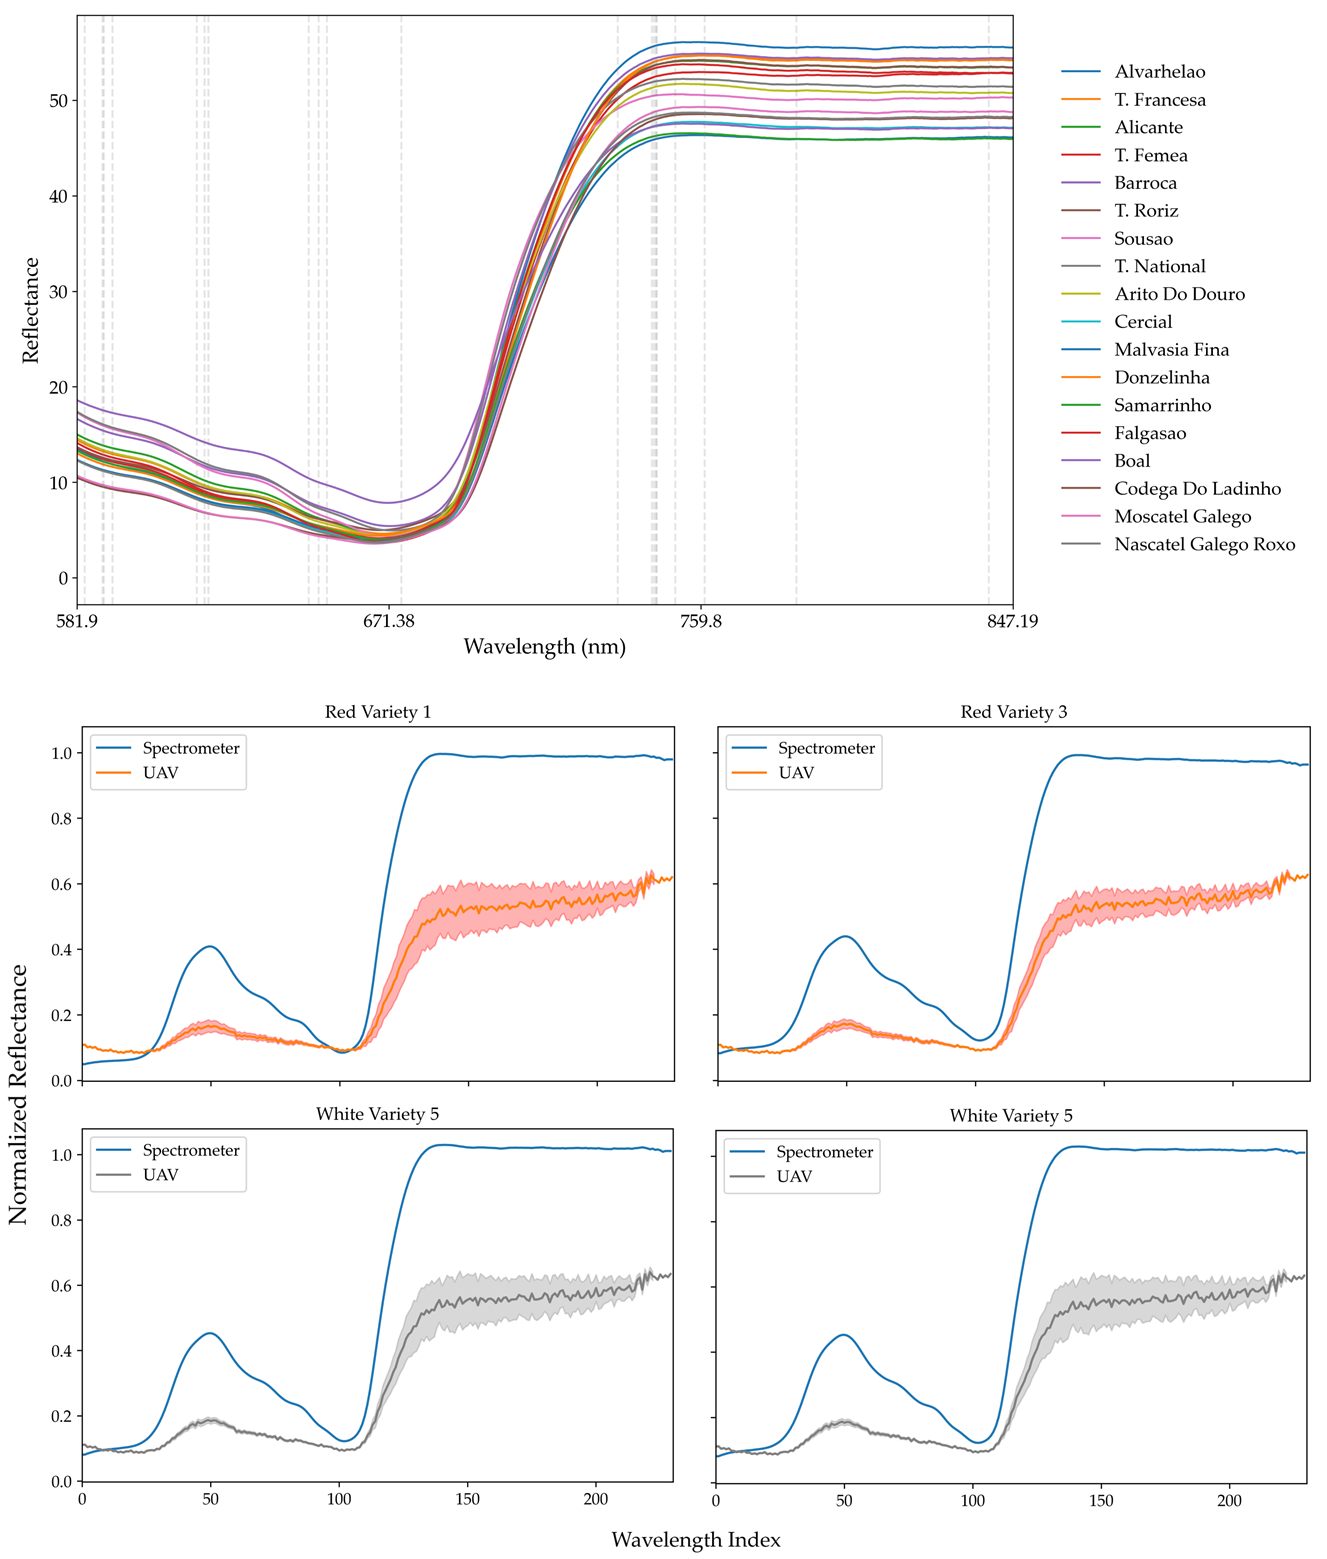
\includegraphics[width=\linewidth]{figs/vineyard_classification/spectrometer_varieties.png}
	\caption{At the top, the average spectrometer signature of every vineyard variety. At the bottom, there is a comparison of the normalized spectrometer and UAV data. Variance is upscaled by a factor of ten for enhancing the visualization.}
	\label{fig:spectrometer_uav_data}
\end{figure}

\section{Processing of UAV data}
\label{sec:vineyard_hyperspectral_processing}

This section briefly describes the process of obtaining reflectance data from raw hyperspectral imagery, which is illustrated in Figure \ref{fig:spectral_view_rectification}. The calculated reflectance is then transformed and standardized to feed a DL network. 

The hyperspectral data was collected using a drone and processed using Headwall SpectralView\texttrademark \hspace{1mm} software. Several swaths were captured for each study area (we refer the reader to Figure \ref{fig:collected_swaths}), and a white sample was marked from the white area in the grayscale tarp. On the other hand, a dark reference was obtained by collecting a hyperspectral sample with the lens cap on before the flight. The sensor exposure and frame period were adjusted before the flight by pointing at a bright reference to avoid clamping samples from white surfaces. The white and dark references were then used to convert the raw data to reflectance. From here, the ortho-rectified swaths were obtained using high-resolution DEMs (25\si{\meter}) from Copernicus' observation program \cite{european_environment_agency_eu_2017} as well as the drone's GPS and IMU data. However, non-ortho-rectified swaths were used for the analyses presented in this paper to work with smaller images and avoid distorting the hyperspectral samples.

\begin{figure*}[ht]
    \centering
    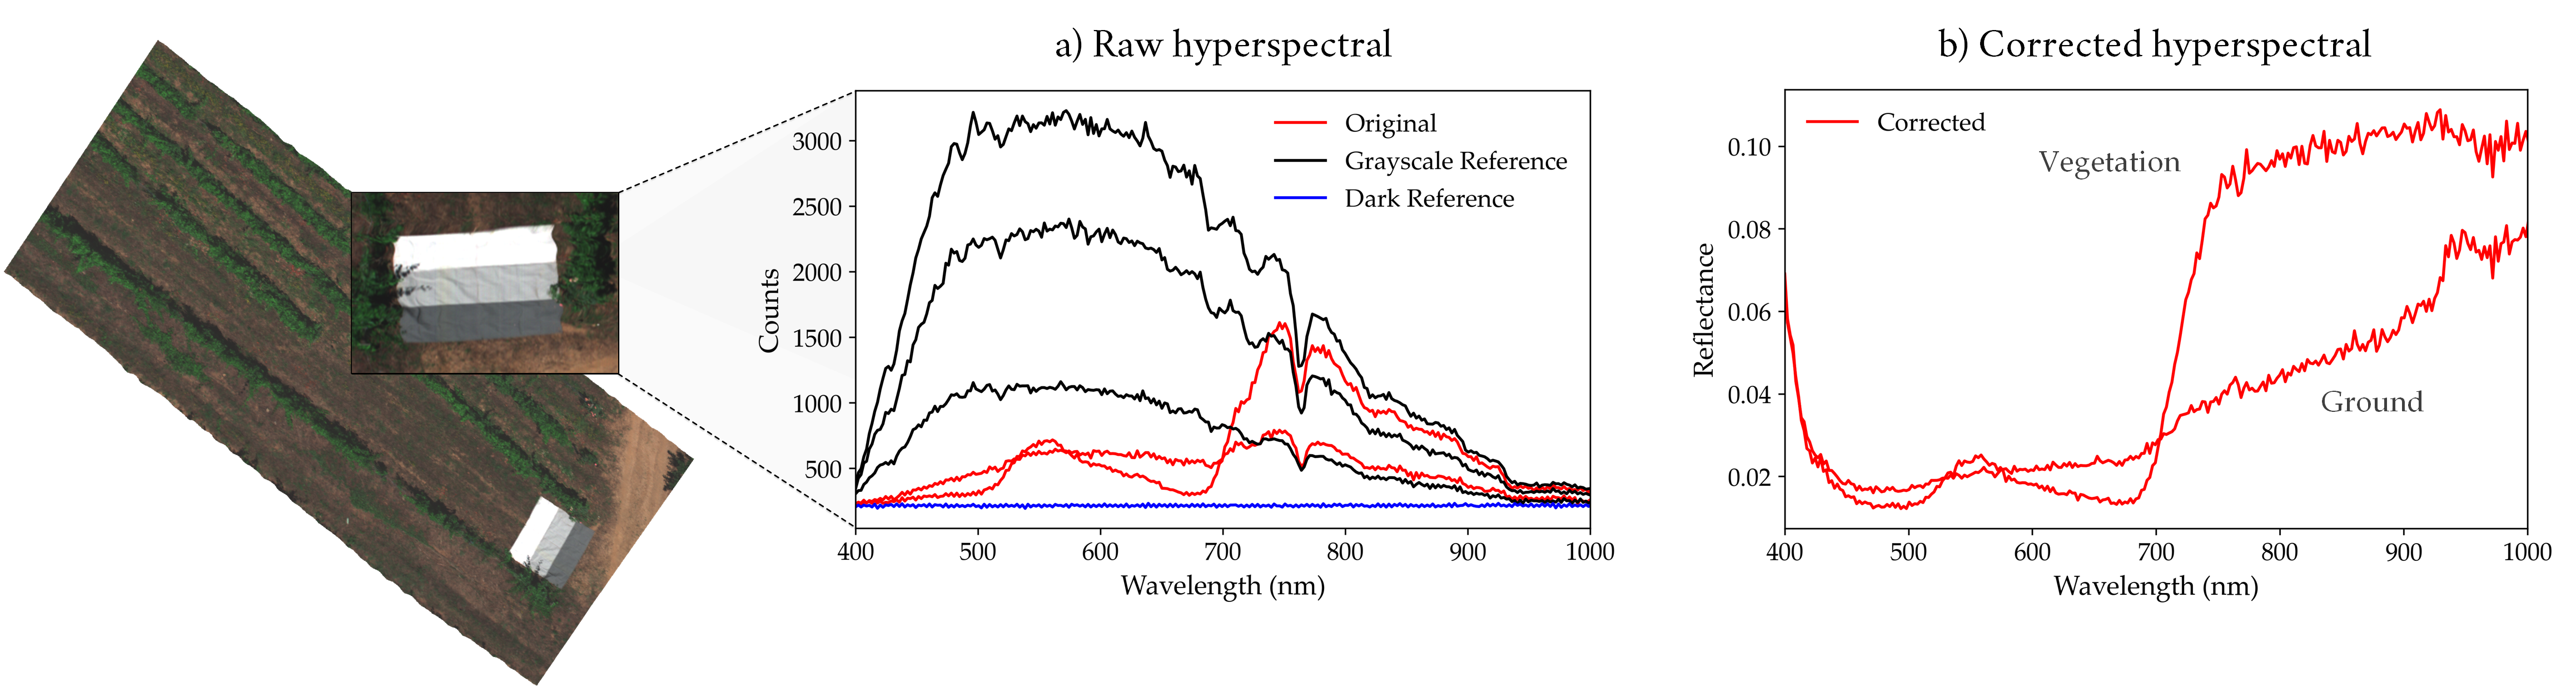
\includegraphics[width=\linewidth]{figs/materials/spectral_view_rectification.png}
	\caption{Conversion of a) hyperspectral DNs into b) reflectance using a white and dark reference. The three gray levels are sampled in a). }
	\label{fig:spectral_view_rectification}
\end{figure*}

In contrast to laboratory data, spectral signatures of hyperspectral swaths' pixels are noisier and fuse several surfaces. Therefore, the classification of these data ought to work under different background surfaces, including soil, low-vegetation and other man-made structures. As proposed in recent work, the material unmixing could be performed with non-negative matrix factorization (NMF). To this end, hyperspectral swaths in reflectance units could be flattened to 1D ($n \gets h \cdot w$) with a dimensionality of $n \times m$, where $m$ is the number of features. Then, this flattened vector could be transformed into weight ($W_{n \times c}$) and component matrices ($C_{c \times m}$), where $c$ is the number of target surfaces (end-members). 

However, the number of materials visible in a single image (or vineyard varieties) is not known in nature. Furthermore, reducing all the varieties into a single vegetation signature leads to poor classification performance, despite $W_i$ being different for each sample. Finally, the signatures observed in the spectrometer could be used to initialize $C$, though it leads to the previous unwanted scenario. Therefore, material unmixing in nature is rather suited for the classification of significantly different signatures rather than performing fine-grained classification. However, the feature space can be transformed and narrowed to a few more representative features, instead of unmixing materials. Methods such as Factor Analysis are also aimed at decomposing $A$ into $W \times C + \Theta$ without the non-negative restriction, with $\Theta$ being the measurement error \cite{bandalos_measurement_2018}. In this regard, FA was shown to perform better than other feature reduction algorithms (e.g., PCA, LDA and Singular Value Decomposition (SVD)).

According to this, hyperspectral samples were processed by 1) splitting train and test samples from the beginning, 2) fitting the FA and standardization solely with training samples and 3) transforming training and test samples with both fitted models. Standardising is applied to remove the mean and scale reflectance to the unit variance. With this approach, the range of input HSI values is restricted in the CNN despite starting values being expected to vary as a result of different sensor exposure, frame period and environmental conditions among distinct flights. On the other hand, HSI noise is tackled by splitting the hyperspectral swaths into patches aimed at classifying pixels using their neighbourhood. Hence, pixels are not significant enough by themselves, although aggregations learnt by kernels help to alleviate the noise.

\section{Automated training}

The classification of vineyard varieties with UAV data can be hardly approached with 1D algorithms due to the high similarity of spectral signatures. In this section, a method based on Deep Learning is described to classify 3D hyperspectral patches. Through this section, the proposed method is tuned to achieve a high generalization performance. 

\begin{figure*}[ht]
    \centering
    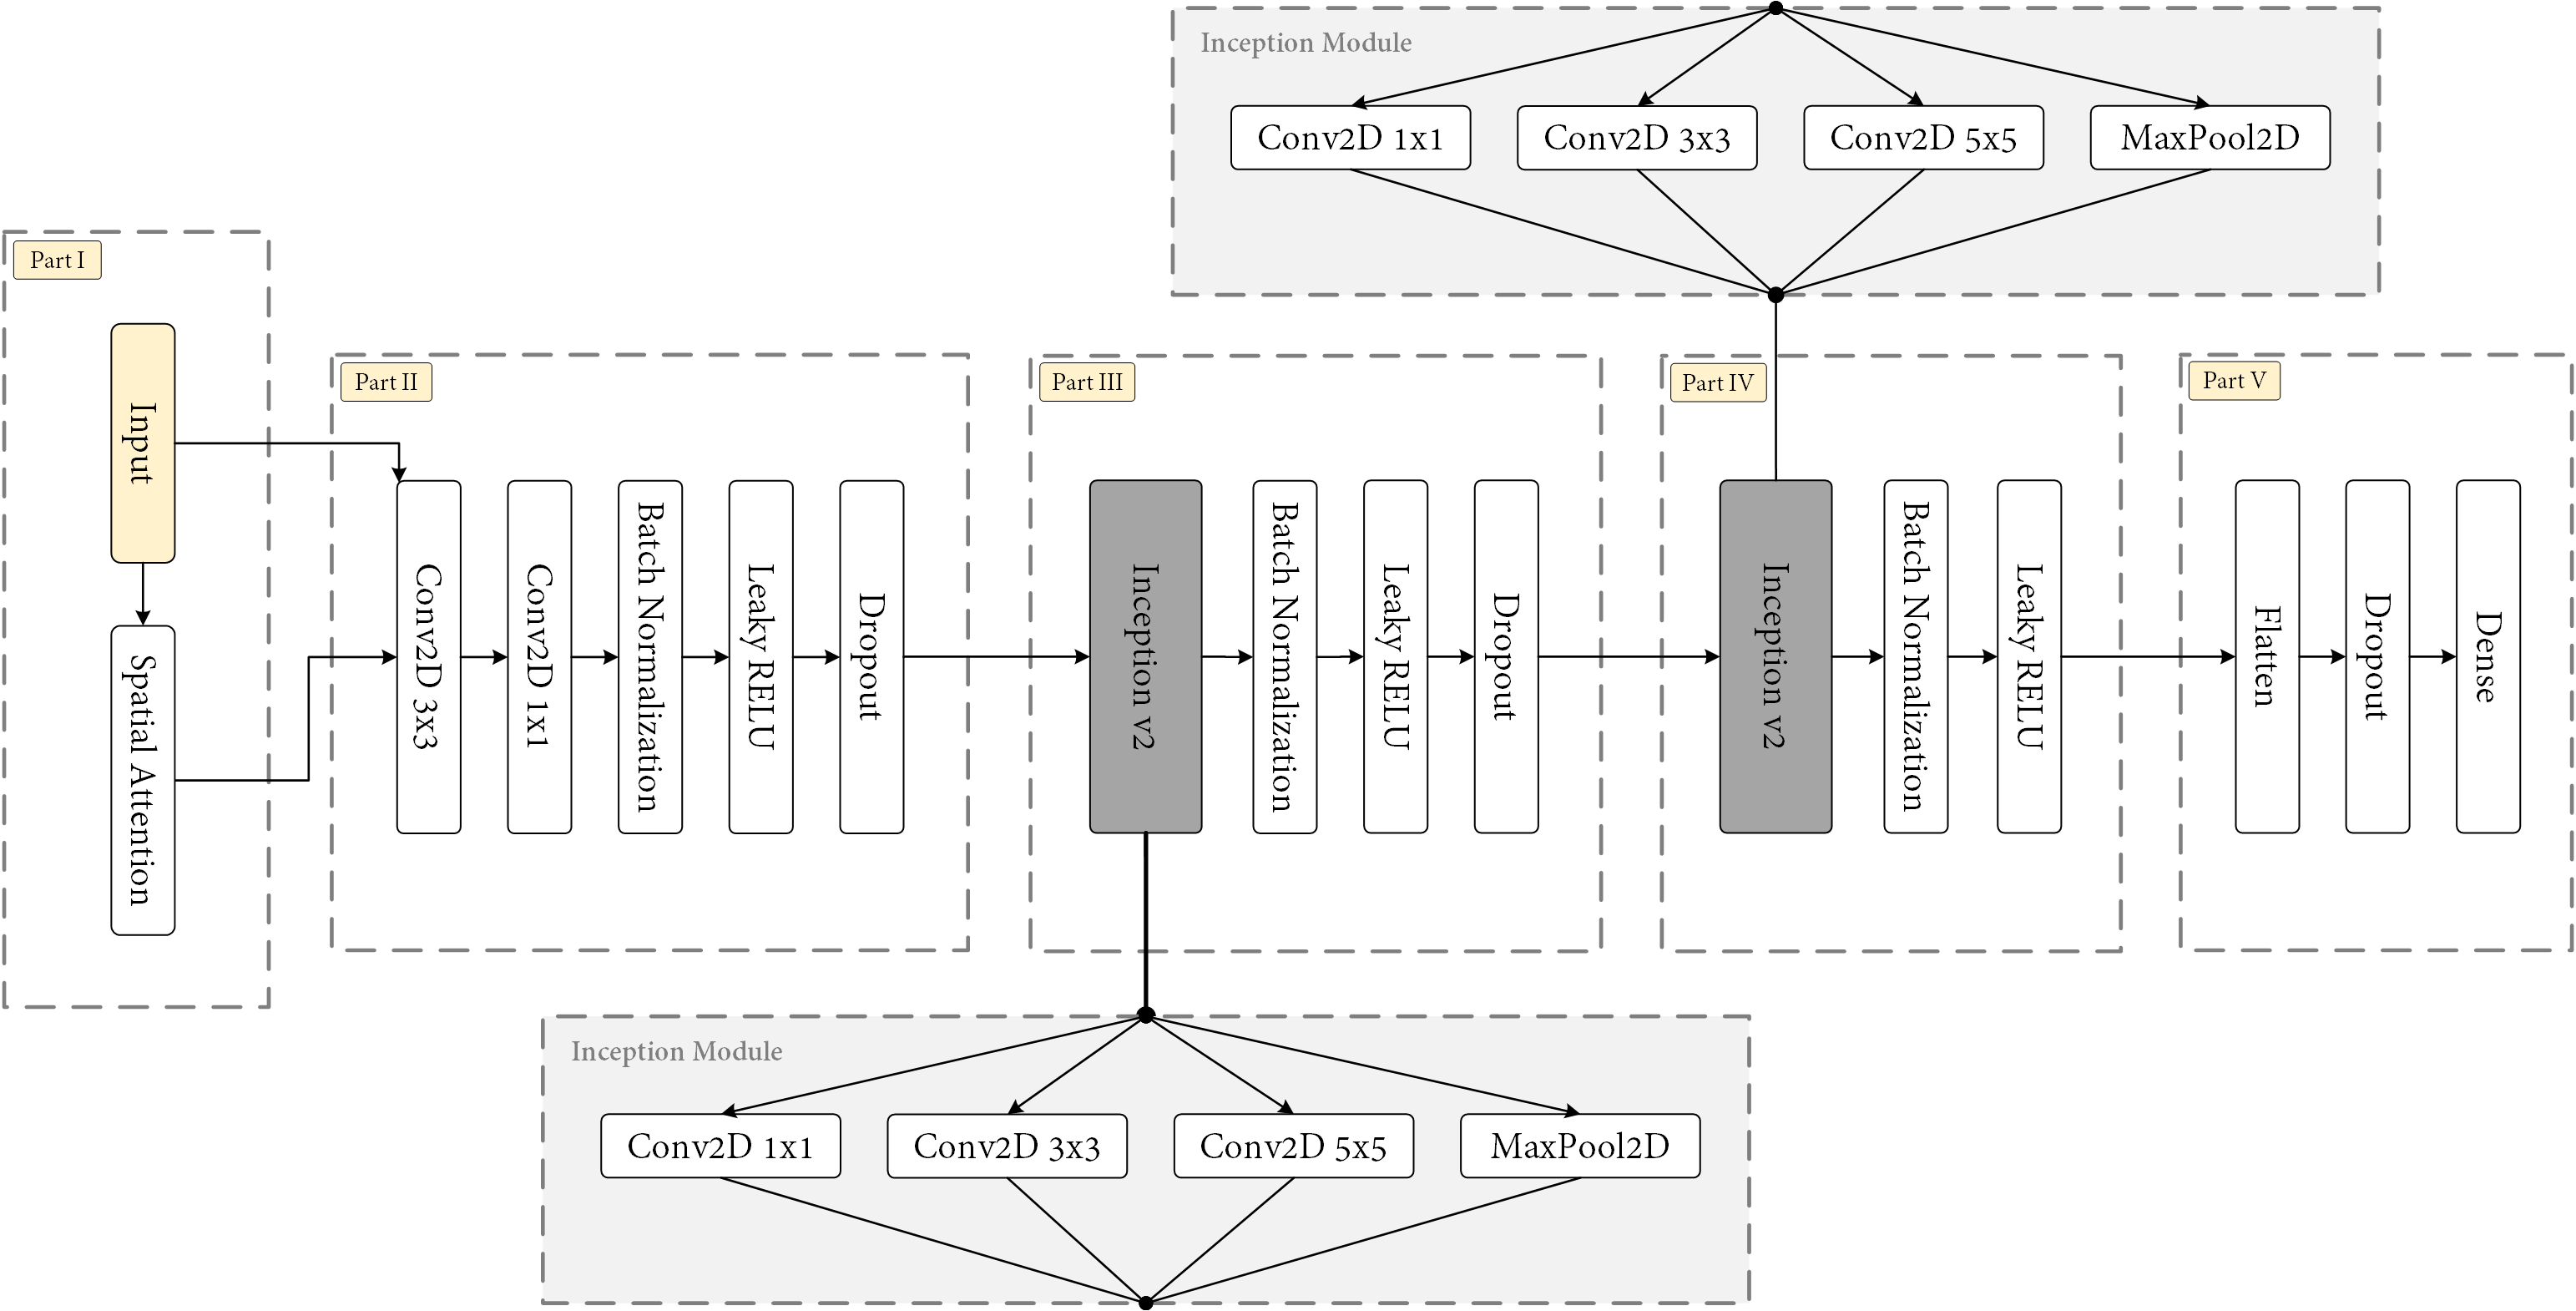
\includegraphics[width=\linewidth]{figs/vineyard_classification/network.png}
	\caption{Overview of dataset preparation. First, a binary mask was generated using the NDVI and rows were organized into different groups to distinguish vineyard classes. Once pixels are processed as described in \nameref{sec:vineyard_hyperspectral_processing}, both reflectance and labels were split into patches. The signatures on the right side show the original and transformed reflectance, including the variance per feature. }
	\label{fig:vineyard_cnn_network}
\end{figure*}

\subsection{Dataset}

The training data is composed of reflectance swaths which are not ortho-rectified, thus diminishing the required memory storage. The Normalized Difference Vegetation Index (NDVI) was then extracted to highlight vegetation in contrast to the ground, and subsequently thresholded to create a binary mask from each swath. These masks were annotated with Sensarea \cite{bertolino_sensarea_2012} by marking each row with a different polygon and colour, according to the variety. Different polygons were labelled with the same colours as some varieties were repeated in several rows. According to this, Table \ref{table:grape_samples} shows the number of collected samples for each variety, including spectrometer and UAV data. 

Then, HSI cubes and masks were split into 3D patches whose size is a matter of discussion in the later experimentation. The window size used in this study is $23 \times 23$ by default, whereas previous work has used patches whose \textit{x} and \textit{y} dimensions range from 7 \cite{roy_attention-based_2021} to 64 \cite{chakraborty_spectralnet_2021}. Only \cite{liu_plant_2022} reported patches of much larger dimensionality ($200 \times 200$). The larger the patch, the deeper can be the network, though it also increases the number of trainable weights, the training time and the amount of data to be transferred into/from the GPU. Configurations using larger patch sizes are more suited to images with notable spatial features, whereas ours ought to be primarily discerned through spectral features. 

Instead of inputting the label of every patch's pixel, they were reduced to a single label corresponding to the centre of an odd-sized patch. Thus, the classification was performed per pixel rather than an overall semantic segmentation. Before being split, pixels were processed to improve the network's performance by reducing spectral dimensionality and shifting the data distribution to have zero mean and unit variance. Regarding feature reduction, spectral bands were transformed and narrowed to $n \gets 30$.

The processing is performed so that it emulates a real-world application. Training and test pixels were first selected through their indices; then, the feature reduction and standard scaler models were fit using only the training dataset. Once adjusted, both training and validation datasets were transformed with both learnt models. None of the fitted models requires the pixel's labels and thus are very convenient for their application in new and unlabelled areas. The resulting dataset is composed of 291,852 and 568,403 patches for red and white varieties, which were split into training (70\%), validation (10\%) and test (20\%) subsets. With this partitioning, a total of 204k samples are used for training on red varieties, whereas 397k are applied to white variety classification.

\begin{figure*}[ht]
    \centering
    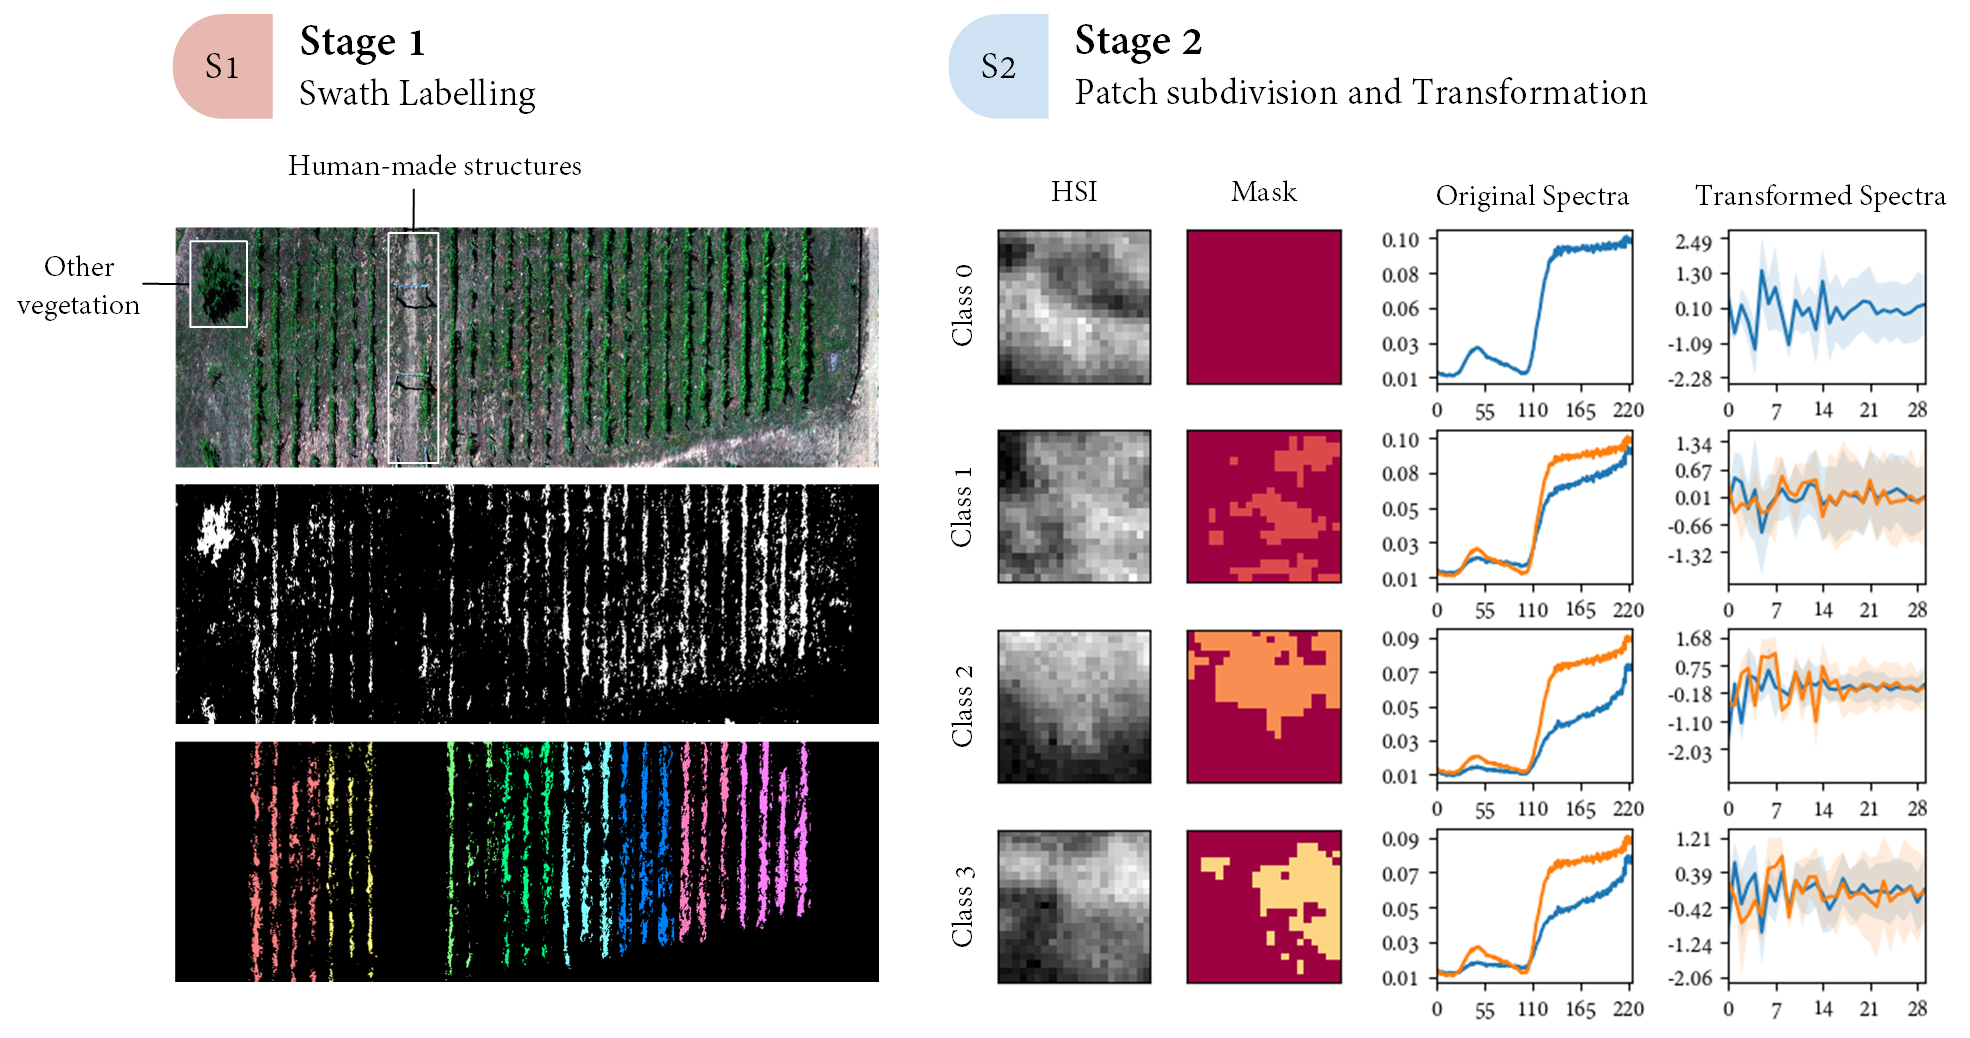
\includegraphics[width=\linewidth]{figs/vineyard_classification/dataset.png}
	\caption{Overview of dataset preparation. First, a binary mask was generated using the NDVI and rows were organized into different groups to distinguish vineyard classes. Once pixels are processed as described in \nameref{sec:uav_processing}, both reflectance and labels were split into patches. The signatures on the right side show the original and transformed reflectance, including the variance per feature. }
	\label{fig:vineyard_dataset}
\end{figure*}

\subsection{Implementation}

In order to make this paper self-contained, a brief introduction about DL is detailed in this section. Firstly, Deep Learning refers to layered representations that evolve in a learning process where they are exposed to input data. Typically, the depth of these models is large enough to automatically transform data and learn meaningful representations of data. Despite these models being able to work over any kind of structured data, even 1D, it is here proposed that one's pixel neighbourhood may help with the phenotyping problem. Convolutional Neural Networks (CNN) have achieved remarkably good results in the computer vision field. Convolutions are designed to learn local features, rather than global, by applying element-wise transformations while sliding over input data. These are defined as rank-3 tensors defined by width, height and depth. The width and height determine how large is the neighbourhood of every element, whereas the depth is the number of different learned filters. Hence, a single filter is applied element-wise to compose a response map from input data, whereas the whole filter stack is known as a feature map. If several convolution operations are concatenated, these evolve from learning low-level details (e.g., edges) to high-level concepts. Since individual filters are applied element-wise, the learnt patterns are invariant to the position within the image \cite{chollet_deep_2021}. However, kernels may not be applied for every element. Instead, information can be compressed using steps greater than one, also known as the stride value. Another key concept in CNN is that not every node is connected, thus partially tackling the overfitting problem. Training and test errors ought to remain similar during training, which implies that the network is not learning the training data (overfitting) or generalizing excessively (underfitting). To avoid both situations, the capacity of the model must be tuned in terms of complexity to generalize and reach low training error.  

Trainable CNN layers are typically defined by a matrix of weights and biases applied over input data, $f(x; w, b)$, with $f$ being an activation function that allows solving non-linear problems. In this work, ReLU and Leaky ReLU have been applied to tackle the vanishing gradient problem, together with batch standardization. The latter operations work similarly to the standardizer applied as a preprocessing stage. On the other hand, $w$ and $b$ are updated during training with the objective of minimizing a loss function comparing ground truth and predicted values for supervised classification. This is done by an optimizer that changes these trainable parameters using the error gradient scaled by the learning rate, $\eta$. The greater $\eta$, the faster is achieved the convergence, though it can also lead to significant oscillations. This process is known as Gradient Descent (GD) \cite{kattenborn_review_2021}. As faster convergence may be necessary at the beginning, the decay and momentum concepts were introduced to downscale $\eta$ during training, thereby omitting abrupt changes.

Besides convolutions and normalization, there exist other layers to narrow data, avoid overfitting and output probabilistic values. The pooling operations, with max and average being the most popular, are aimed at downsampling input data. Dropout layers are used as a mechanism to introduce some noise into the training by zeroing out some output values, thus getting rid of happenstance patterns. Weight regularization also seeks to make the model simpler by forcing the weights to be small. Finally, the output units of the model are aimed at transforming features to complete the classification task. For a multi-label problem, the Softmax represents the probability distribution of a variable with $n$ possible values. 

The kind of problem and label representation are coupled with the cross-entropy function measuring the error. Sample labels were not hot-encoded to reduce storage footprint, and therefore, a sparse categorical cross-entropy as defined in Equation \ref{eq:crossentropy} is used for training in a multi-class problem. Otherwise, hot-encoding requires transforming labels into binary vectors of size $c$ that activate the indices of the sample label(s), with $c$ being the number of unique labels. 
\begin{align*}
    L_{\textit{CE}} = -\ln{\left(\hat{y}\left[y\right]\right)}
    \numberthis \label{eq:crossentropy}
\end{align*}
where $\hat{y}$ is the model's output as a vector of size $c$ with $\hat{y}\left[i\right], i \in \left[0, c - 1\right]$ indicating the probability of the sample to belong to the i-th class, and $y$ is the ground truth given by an integer value.

\subsection{Architecture and training}

Several architectures were checked over both datasets, transitioning from networks with a few layers to the network proposed in Figure \ref{fig:vineyard_cnn_network}. Hyper-parameter tunning was also used to define the best values for dropout, activation and convolutional layers, including the number of filters, the percentage of zeroed weights, or the gradient of Leaky ReLU activation. Similarly, the final activation was also checked despite Softmax being usual for multi-class output. 

The input of the network is a single patch of size $23 \times 23$ and 30 bands. The spatial attention layer proposed by \cite{xue_attention-based_2021} is appended as an additional layer that is shown to help with the classification. The original paper proposed first and second-order pooling before and after the spatial attention module to transform the original features as we did with FA. Also, the inputted images are augmented prior to training, rather than using a single patch with each rotation being applied with a probability.

Attention-based kernels have been recently used for HSI classification to provide more discriminative spectral-spatial features from input data. \cite{xue_attention-based_2021} applied attention-based as a link among the first data transformation, coined as a first-order feature operator, and a second-order kernel. \cite{roy_attention-based_2021} used an attention-based kernel in a similar fashion to \cite{xue_attention-based_2021}, though this one was replicated throughout the network pipeline. It was also part of a residual network where the input is simultaneously processed through 1) an attention kernel and 2) convolutional layers. The outputs of both pipelines are then concatenated at the ending point of each network's block. 

In this work, the attention-based a) kernel of \cite{xue_attention-based_2021} is applied over input data and the result is concatenated in $z$ with the original inputted data. The first operation in the attention-based thread is to normalize the data, from which the kernel will learn the weights. Such a kernel is a correlation matrix that learns the cosine distance between the central pixel and the neighbours. Then, learned weights are normalized through a softmax function that is shown to provide better convergence. With this in mind, the attention-based can be formulated as follows:
\newcommand{\inputMatrix}{{\mathcal{P}_{\textit{norm}}}^{M^2 \times B}}
\newcommand{\inputMatrixTranspose}{\left({\mathcal{P}_{\textit{norm}}}^{M^2 \times B}\right)^\intercal}
\begin{align*}
    \inputMatrix &\gets l_2 (\mathcal{P}^{M^2 \times B}) \numberthis \label{eq:spatial_attention_01}\\
    \mathcal{S}^{M^2 \times M^2} &\gets \left[\inputMatrix \inputMatrixTranspose\right] \numberthis \label{eq:spatial_attention_02}\\
    {\mathcal{S}_{central}}^{M^2 \times 1} &\gets \left[{{\mathcal{S}}_{\lfloor{\frac{M}{2}\rfloor}}}^{M^2}\right]^\intercal \mathcal{K}^{M^2 \times 1} \numberthis \label{eq:spatial_attention_03}\\
    \mathcal{SA}^{M^2} &\gets \mathcal{S}^{M^2 \times M^2} \mathcal{K}^{M^2 \times 1} + \mathcal{B}^{M^2 \times 1} \numberthis \label{eq:spatial_attention_04}\\
    {\mathcal{P}_{\mathcal{SA}}}^{M^2 \times B} &\gets \textit{softmax}(\mathcal{SA}^{M^2}) \cdot \mathcal{P}^{M^2 \times B} \numberthis \label{eq:spatial_attention_05} 
\end{align*}
where $l_2$ refers to L2 normalization, $\mathcal{P}^{M^2 \times B}$ is a 3D patch resized from $\mathcal{P}^{M \times M \times B}$, $\mathcal{S}$, $\mathcal{S}_{\textit{central}}$ as well as $\mathcal{SA}$ are intermediate states and $\mathcal{P}_{\mathcal{SA}}$ is the result that is later concatenated with the original form.

Then, the second module is aimed at extracting both spatial and spectral features, as proposed by \cite{pan_spectral-spatial_2020}. The first convolutional layer is applied pixel-wise with a kernel of size 1 and thus operates by extracting patterns on the $z$-axis. It is used prior to kernels of larger size to compute reductions. Then, the second convolutional layer extracts spatial features over previously extracted filters. The kernel size is only 3 since deeper layers will operate over larger neighbourhoods.

\newcommand{\kernelSize}[1]{#1 $\times$ #1}
\newcommand{\outputSize}[2]{#1 $\times$ #1 $\times$ #2}
\renewcommand{\arraystretch}{1}
\begin{table*}
\centering
\caption{Layer specifications of the proposed network. Inception is simply named, but its layers were not expanded here to make this table more readable. \\ }
\label{table:cnn_architecture}
\begin{tabular}{lllll}
\toprule
Part & Layer & Kernel size & Strides & Output size\\
\midrule
\multirow{3}{*}{I} & Input & & & \outputSize{23}{30}\\
& Spatial Attention & & & \outputSize{23}{30}\\
& Concatenate & & & \outputSize{23}{60}\\
\midrule
\multirow{5}{*}{II} & Conv2D & \kernelSize{1} & 1 & \outputSize{23}{16}\\
& Conv2D & \kernelSize{3} & 2 & \outputSize{12}{16}\\
& Leaky ReLU ($\alpha \gets 0.1$) & & & \outputSize{12}{16}\\
& Batch normalization & & & \outputSize{12}{16}\\
& Dropout (0.2) & & & \outputSize{12}{16}\\
\midrule
\multirow{5}{*}{III} & Inception v2 & & 1 (Conv2D $1 \times 1$), 2 & \outputSize{6}{112} \\
& Batch normalization & & & \outputSize{6}{112}\\
& Leaky ReLU ($\alpha \gets 0.1$) & & & \outputSize{6}{112}\\
& Dropout (0.4) & & & \outputSize{6}{112}\\
\midrule
\multirow{5}{*}{IV} & Inception v2 & & 1 (Conv2D $1 \times 1$), 2 & \outputSize{3}{288}\\
& Batch normalization & & & \outputSize{3}{288}\\
& Leaky ReLU ($\alpha \gets 0.1$) & & & \outputSize{3}{288}\\
& Flatten & & & 2592\\
& Dropout (0.2) & & & 2592\\
\midrule
\multirow{1}{*}{V} & Softmax & & & 9 (Red), 11 (White)\\
\midrule
\multicolumn{5}{c}{\#Trainable parameters: 395643}\\
\multicolumn{5}{c}{\#Non-trainable parameters: 992}\\
\multicolumn{5}{c}{\#Parameters: 396635}\\
\bottomrule
\end{tabular}
\end{table*}
\renewcommand{\arraystretch}{1}

Two similar blocks are included as Part III and Part IV in Figure \ref{fig:vineyard_cnn_network}. Both share the same structure: Inception block, normalization, activation and dropout. It s a frequent follow-up of convolutional layers \cite{li_faster_2022, xue_attention-based_2021}, with dropout being greater (0.4) for middle layers than the last and initial layers (0.2). Instead of using max-pooling to downsample the network, strides in convolutional layers were observed to perform better. Thus, strides of size 2 were used in spatial-based CNN layers. The network specifications are shown in Table \ref{table:cnn_architecture}.

The Inception block was first proposed by \cite{szegedy_going_2014}. The first proposal consisted of a module with four parallel layers later concatenated: convolutional layers with different kernel sizes (1 for spectral features and 3 and 5 to obtain aggregations from surrounding pixels), and a max-pooling layer that works directly over input data. Accordingly, a response map with a large number of filters is obtained. The importance of each of them is determined by the following layers that will again downsample data. However, at the time this layout was considered to be prohibitive if the input layer has a large number of filters, especially for kernels of larger size. Therefore, $1\times1$ convolutions aimed at reducing data were attached before each one of the Inception threads (max-pool and convolutions with $\kappa > 1$). In this work, both proposals were used: the naïve is checked in the experimentation to increase the network's capacity, whereas the second is part of the proposed network. The latter compresses spatial data even more and is following connected to the network output. The code showing the skeleton of the proposed network is shown in Code \ref{code:vineyardmodel}.

\lstinputlisting[language=python, caption={The proposed CNN network aimed at classifying different vineyard varieties.}, label=code:vineyardmodel]{code/vineyard_allopezr2d_skeleton.py}

Finally, the model is fitted with training data and its performance is assessed with validation samples. For supervised problems like ours, data is composed of both samples and ground truth. In this work, the training samples were split into several sets according to the hardware limitations, and the model was iteratively trained with a significant number of iterations for every set ($\varepsilon \gets 100$). Besides mitigating storage limitations, this leave-p-out cross-validation also helps to generalize by not training over the complete dataset. Furthermore, each one of these clusters is further split into small batches during a single iteration. The batch size must be large enough to include a balanced representation of samples. In this work, the batch size was set to $2^{10}$. This phase can be terminated early if no improvements are observed during $t$ epochs, with $t \gets 20$ in this work.

\subsection{Data sampling and regularization}

It can be observed from Figure \ref{fig:vineyard_dataset} that the dataset is clearly not balanced. The number of ground-labelled batches is considerably larger if uniformly sampled, whereas vineyard rows also differ in length and so does the number of examples for each variety. Instead of generating new feasible batches to upsample, a subset was obtained with different techniques. These range from randomization to clustering, with the second returning better results. This approach leads to over 14K examples for every vineyard class in the first round. To avoid omitting samples from wider vineyard rows, the rest of the non-ground samples are used for training in a second iteration. Hence, the second phase starts from a network trained with a balanced dataset. In any case, the CNN is watched with a callback that saves the current best model and prevents saving an overfitted model.

To summarize, the sampling strategy is the following. First, the preprocessing transformations are fit to the training samples, $\mathcal{X}$. Then, the whole HSI cube, $\mathcal{B}$, is transformed according to the models learnt with $\mathcal{X}$, allowing us to simulate the classification of new, non-labelled, samples in nature. After that, 3) HSI cubes are split into squared-odd-sized patches ($\mathcal{H}^{W \times H \times D} \rightarrow \mathcal{P}^{S \times S \times D}$ with $S \in A_{\mathcal{O}}$), 4) patches' labels are reduced into the label of the central pixel ($f(\mathcal{P}_{\texttt{label}}^{S \times S}) \rightarrow \mathcal{P}_{\texttt{label}}^{1 \times 1}$), 5) the dataset is balanced with clustered downsampling ($\mathcal{P} \rightarrow \mathcal{B}$) and 6) $\mathcal{B}$ is divided into train $\mathcal{B}_{0.7} \rightarrow \mathcal{X}$ and test datasets $\mathcal{B}_{0.3} \rightarrow \mathcal{T}$, where the former is again split during training to obtain the validation dataset ($10\%$ of $\mathcal{B}$).

From both datasets (balanced and second-round vegetation), batches were augmented by performing rotations and orientation flips so that learn features are invariant to the flight's positioning conditions (see Figure \ref{fig:patch_augmentation}). With this approach, the dataset was augmented by $\times 5$. Hence, the regularization was controlled by the proposed downsampling and augmentation sequences. Several considerations were also taken into account during the CNN design: 1) the CNN must not have a large number of trainable parameters to avoid overfitting, and a sufficient number to cope with underfitting, and 2) dropout layers were included to randomly reset some output weights and thus lead to proper generalization.

\begin{figure}[ht]
    \centering
    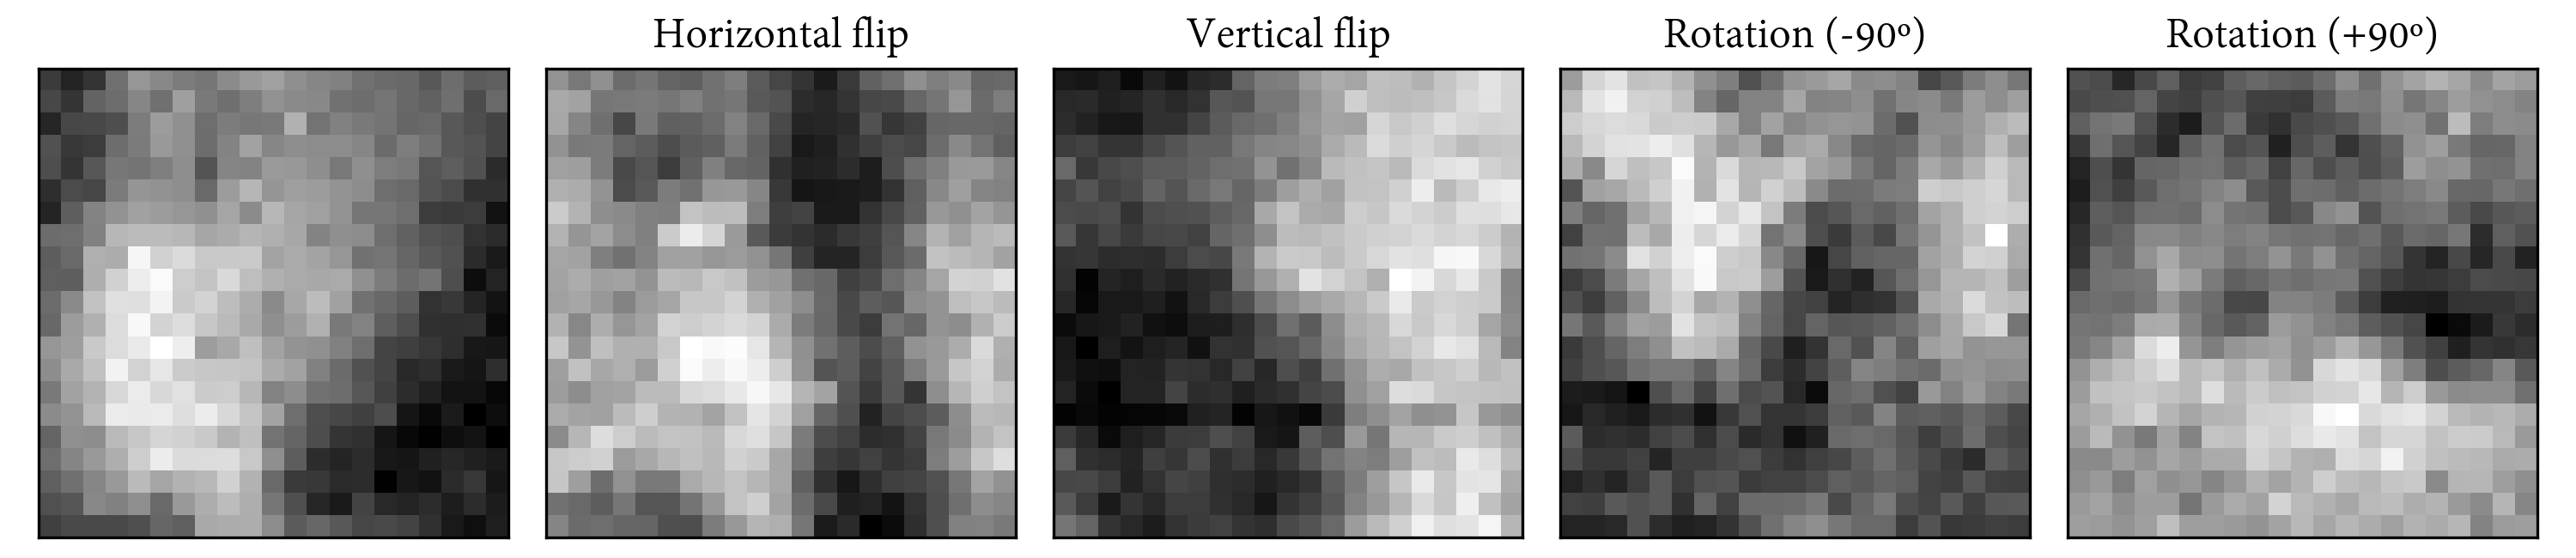
\includegraphics[width=\linewidth]{figs/vineyard_classification/patch_augmentation.png}
	\caption{Augmentation of a single hyperspectral patch ($23\times23$). }
	\label{fig:patch_augmentation}
\end{figure}

\section{Experimentation and analysis}

\begin{figure*}[bht]
    \centering
    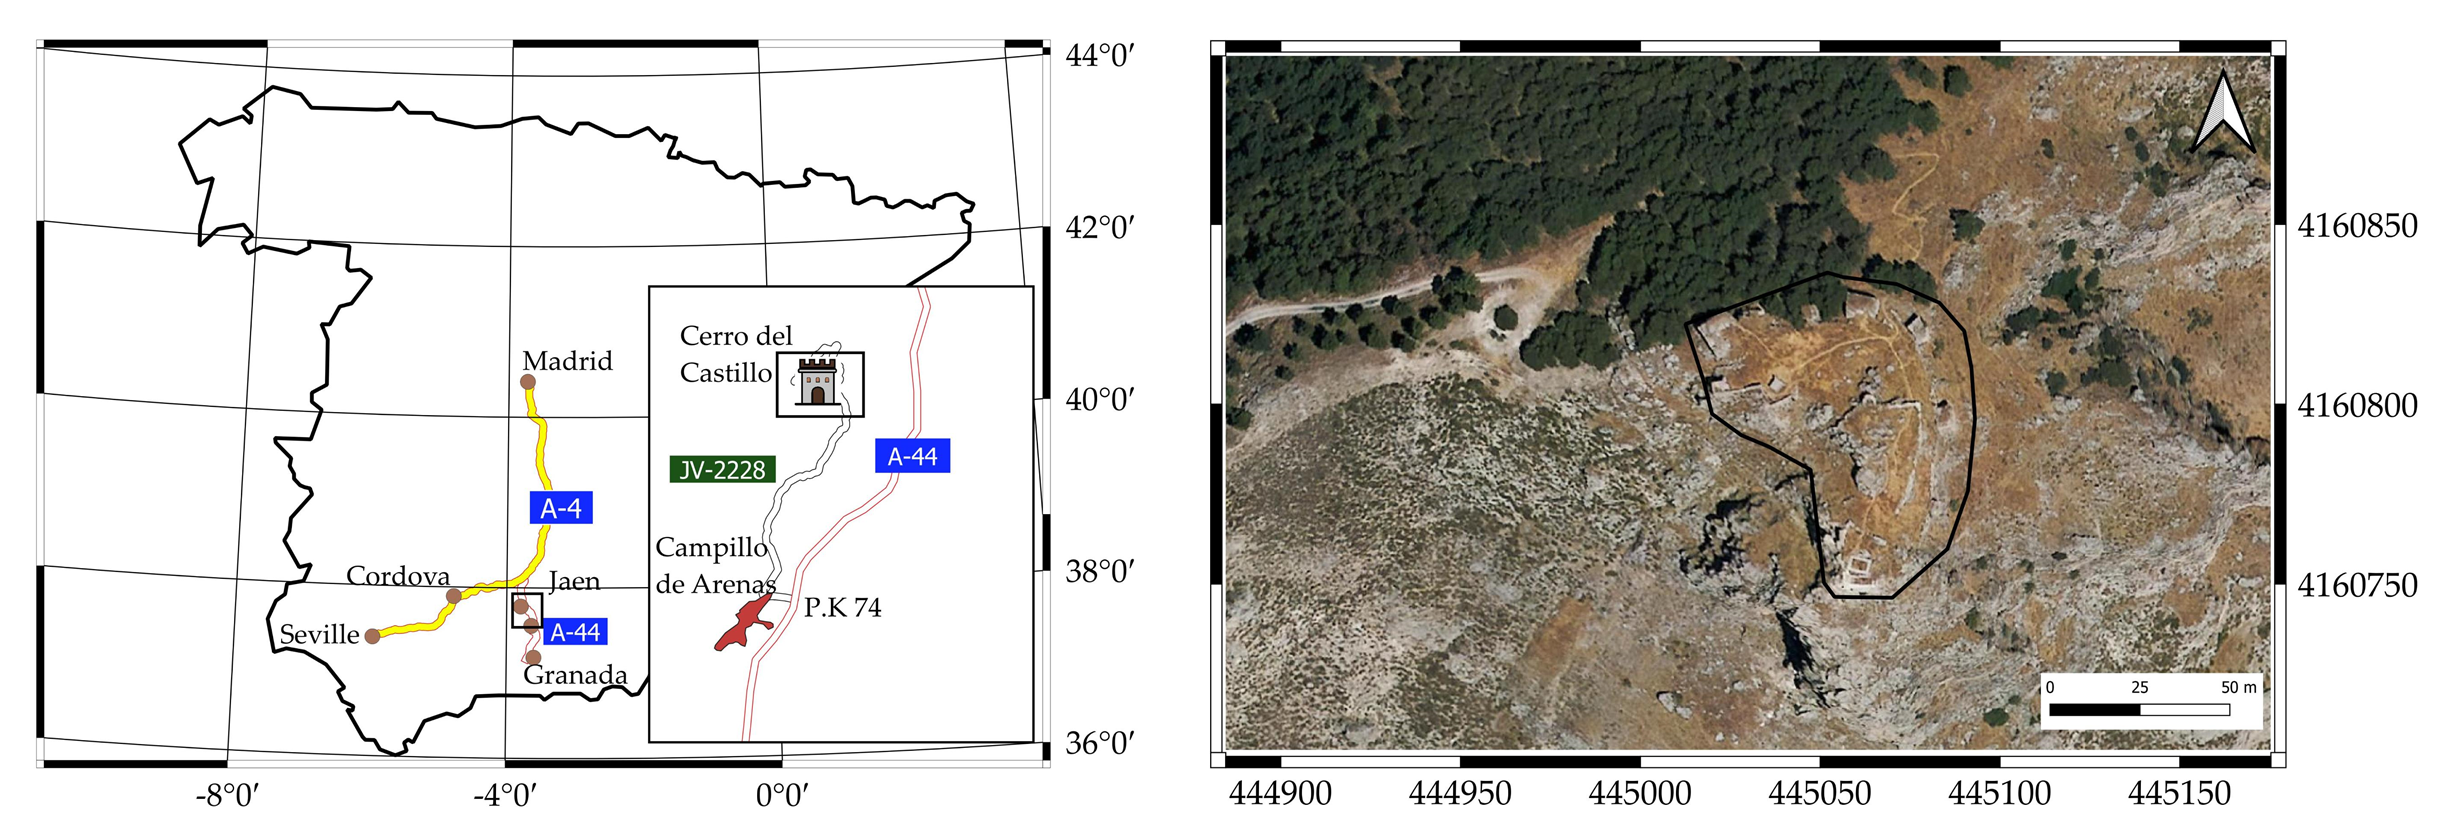
\includegraphics[width=\linewidth]{figs/vineyard_classification/study_area.png}
	\caption{Overview of the areas surveyed with UAV hyperspectral imaging for the classification task. Two different vineyard crops are depicted according to their main variety: a) red and b) white. }
	\label{fig:vineyard_study_area}
\end{figure*}

A brief explanation of the study area and sensors is first provided in this section; then, the performance of the proposed network is evaluated over multiple hyperspectral swaths collected in the two surveyed areas. Results are presented in terms of overall accuracy (OA), average accuracy (AA), statistical kappa ($\kappa$) and f1-score. The first shows the percentage of correctly classified samples, the AA represents the average class-wise accuracy, the $\kappa$ coefficient is the degree of agreement between the classification results and the ground truth, and finally, the f1-score measures the model's precision by leveraging both precision and recall metrics. Several representative neural networks are compared with our method: LtCNN \cite{liu_plant_2022}, JigsawHSI \cite{moraga_jigsawhsi_2022}, SpectralNET \cite{chakraborty_spectralnet_2021}, HybridSN \cite{roy_hybridsn_2020}, Nezami et al. \cite{nezami_tree_2020} and A-SPN \cite{xue_attention-based_2021}. From these, only a few address airborne-sensing imagery \cite{liu_plant_2022}, whereas the rest are focused on satellite data. Hence, several considerations must be addressed: 1) some of these manuscripts apply different transformations to the input data and 2) the number of spectral bands also differ from our sensing tool. Therefore, the preprocessing pipeline was selected as the one providing better performance over our input data, either our pipeline or the one proposed in the reference work. However, FA showed a higher performance for every network if input data was transformed according to this fitting method, rather than the following: 
\begin{itemize}
    \item Nezami et al. \cite{nezami_tree_2020}, Liu et al. \cite{liu_plant_2022} (LtCNN) used the corrected reflectance with no preprocessing. 
    \item Moraga and Duzgun \cite{moraga_jigsawhsi_2022} (JigsawHSI) used PCA, FA, SVD and NMF with 9-12 final features.
    \item Liu et al. \cite{liu_plant_2022} (A-SPN) and \cite{roy_hybridsn_2020} (HybridSN) used PCA to transform reflectance with $n \gets 15, 30$, respectively, whereas $n$ is unknown for \cite{xue_attention-based_2021}.
    \item Chakraborty and Trehan \cite{chakraborty_spectralnet_2021} (SpectralNet) used FA with only 3 features.
\end{itemize}

Regarding implementation, all the tests were performed on a PC with AMD Ryzen Threadripper 3970X 3.6 GHz, 256 GB RAM, Nvidia RTX A6000 GPU and Windows 10 OS. The proposed CNN as well as the compared networks were implemented with Keras (version 2.10.0) and TensorFlow (version 2.10.1) in Python. CUDA 11.8 and CuNN 8.6 were installed to reduce the fitting time. Not every network from previous work could be applied as published; for example, LtCNN is designed for large image patches ($200\times200$) and thus convolutional striding and MaxPooling cannot be applied when patches reach a size of $1\times1$. For LtCNN \cite{lu_hyperspectral_2022}, kernel size and max pooling's strides were reduced as depicted in Figure \ref{fig:lt_cnn}. The rest of networks are also documented, from Figure \ref{fig:aspn_cnn} to Figure \ref{fig:hybridsn_cnn}.

\subsection{Study area}

The vineyards used as study areas in this work are situated in the Northern region of Portugal, specifically in Vila Real \ref{fig:vineyard_study_area}). Each vineyard plot is dedicated to either red or white grapevine variants, and each grapevine variety is cultivated in one or more contiguous rows. Data acquisition occurred in two ways: 1) by gathering leaves from each row, directly on the field, and 2) by conducting a UAV flight, which is described subsequently. The initial outcomes were analyzed in a laboratory setting, while the second survey was dedicated to collecting HSI swaths.

\subsection{Material}

The M600 hexacopter equipped with a Nano-Hyperspec from Headwall was used for the UAV flight. The flight was planned using Universal Ground Control Station at an altitude of 50 \si{\meter} with a 40\% side overlap. 5 and 8 swaths were obtained for red and white grapevine varieties, respectively, as depicted in Figure \ref{fig:vineyard_swaths}. The leaves collected were analyzed at the University of Trás-os Montes e Alto Douro (UTAD) using a spectrometer, where reflectivity was acquired by sampling the front and back of each leaf under controlled illumination. The first and last reflectance samples were discarded since they were noisier, thus narrowing down the spectral interval from 187.63-1100.35 \si{\nano\meter} to 450-950 \si{\nano\meter}. Even after applying filters, some spectral signatures differed significantly from the expected average profile ($\mu$) and were removed based on the distance calculation from $\mu$. Table \ref{table:grape_samples} provides a summary of the collected grape leaf samples.

\subsection{Impact of window size}

The patch size is one, if not the most relevant, parameter concerning the network architecture. Larger patches are assumed to also work as irrelevant spatial features can be zeroed out. However, it also comes at the expense of increasing the training time. On the contrary, lower patches come at the risk of not being sufficient for classifying samples as accurately as done by the proposed network. Figure \ref{fig:window_size_test} shows the whole battery of metrics obtained with patch sizes ranging from 9 to 31. On the other hand, Figure \ref{fig:time_capacity_test} emphasizes the training time, in minutes, and the dimensionality of the network. According to the obtained results, patches have been split with dimensionality 23 to balance network capacity and accuracy, despite higher patch size achieving slightly better results. Accordingly, the highest patch size reached an OA of 99.63\% for red varieties, whereas the lowest reached 86\% (9). On the other hand, the selected dimensionality achieves an OA of 99.37\%. Regarding white varieties, the proposed network did not achieve better results with larger patch sizes. The best OA was obtained using patches of size 23, whereas the lowest was reached using the lowest patch size, 9, with an OA of 85\%.

\begin{figure*}[ht]
    \centering
    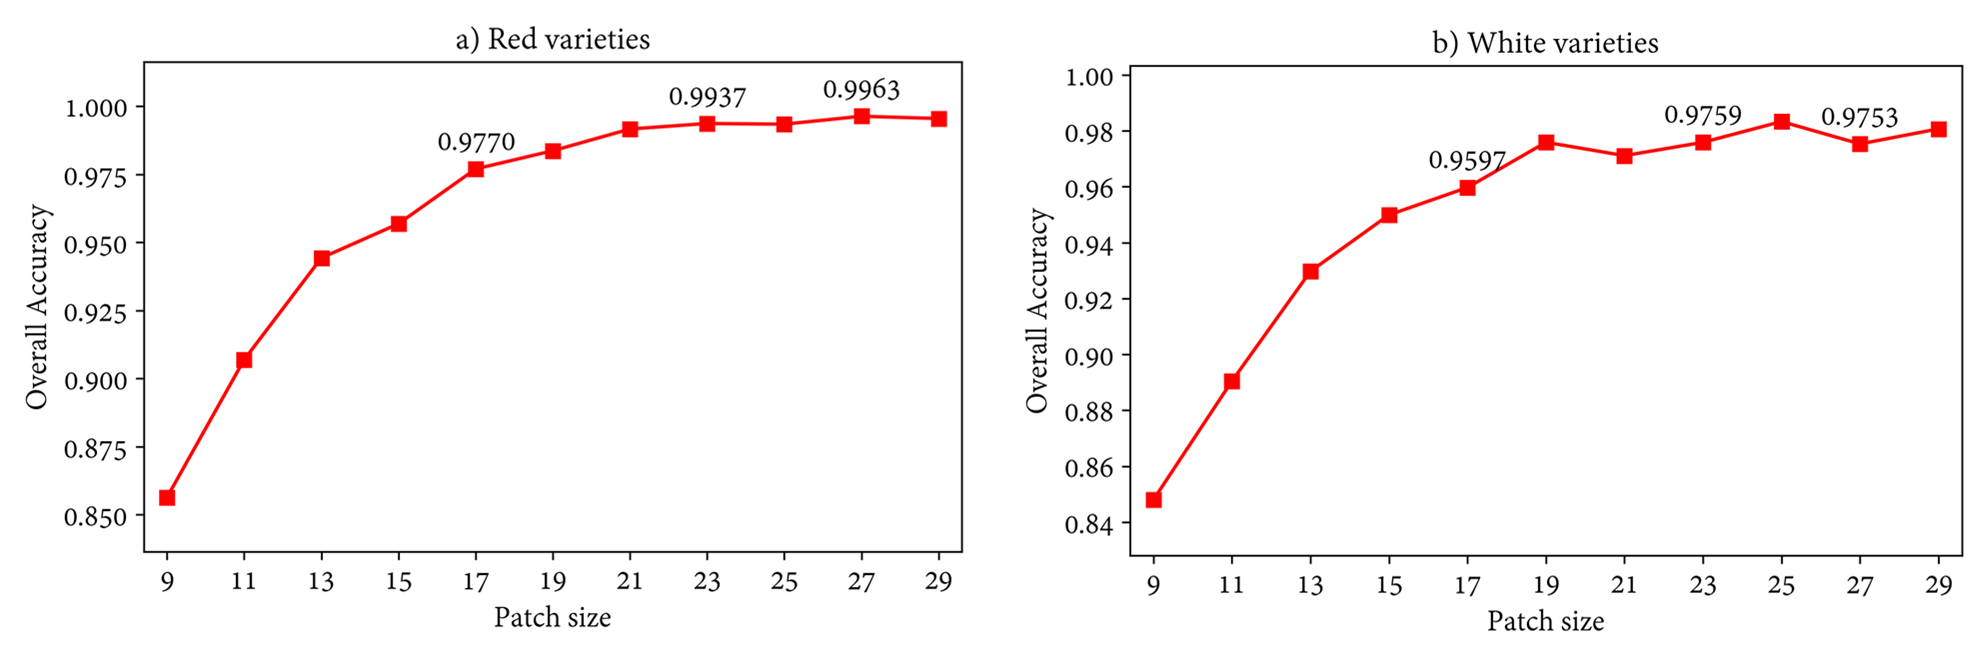
\includegraphics[width=\linewidth]{figs/vineyard_classification/window_size_test.png}
	\caption{Overall accuracy obtained for patches of different sizes, from 9 to 31. }
	\label{fig:window_size_test}
\end{figure*}

\begin{figure*}[ht]
    \centering
    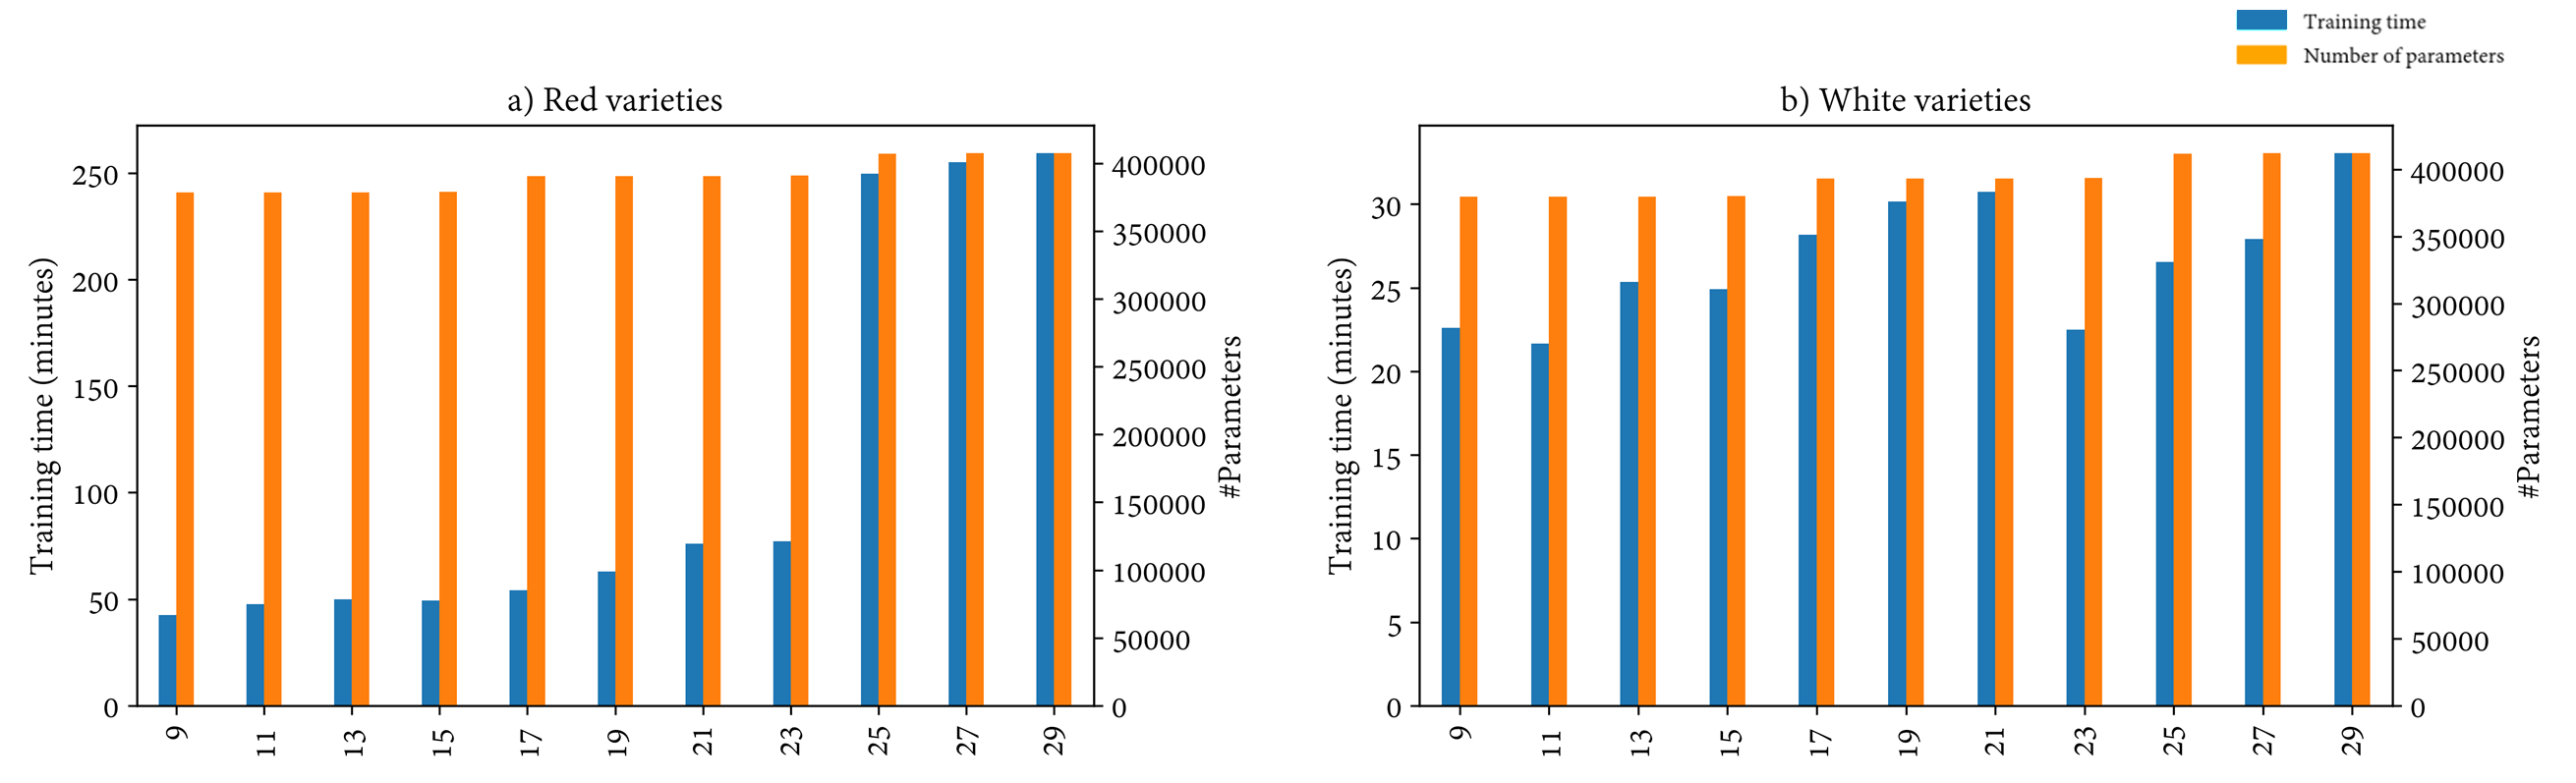
\includegraphics[width=\linewidth]{figs/vineyard_classification/time_capacity.png}
	\caption{Training time, in minutes, and number of parameters as the window size increases. }
	\label{fig:time_capacity_test}
\end{figure*}

\subsection{Ablation study}

The proposed network is intended to be validated in this section by removing some of the network features, while the rest remain unchanged. The proposed changes are the following:
\begin{marginfigure}[1.cm]
    \centering
    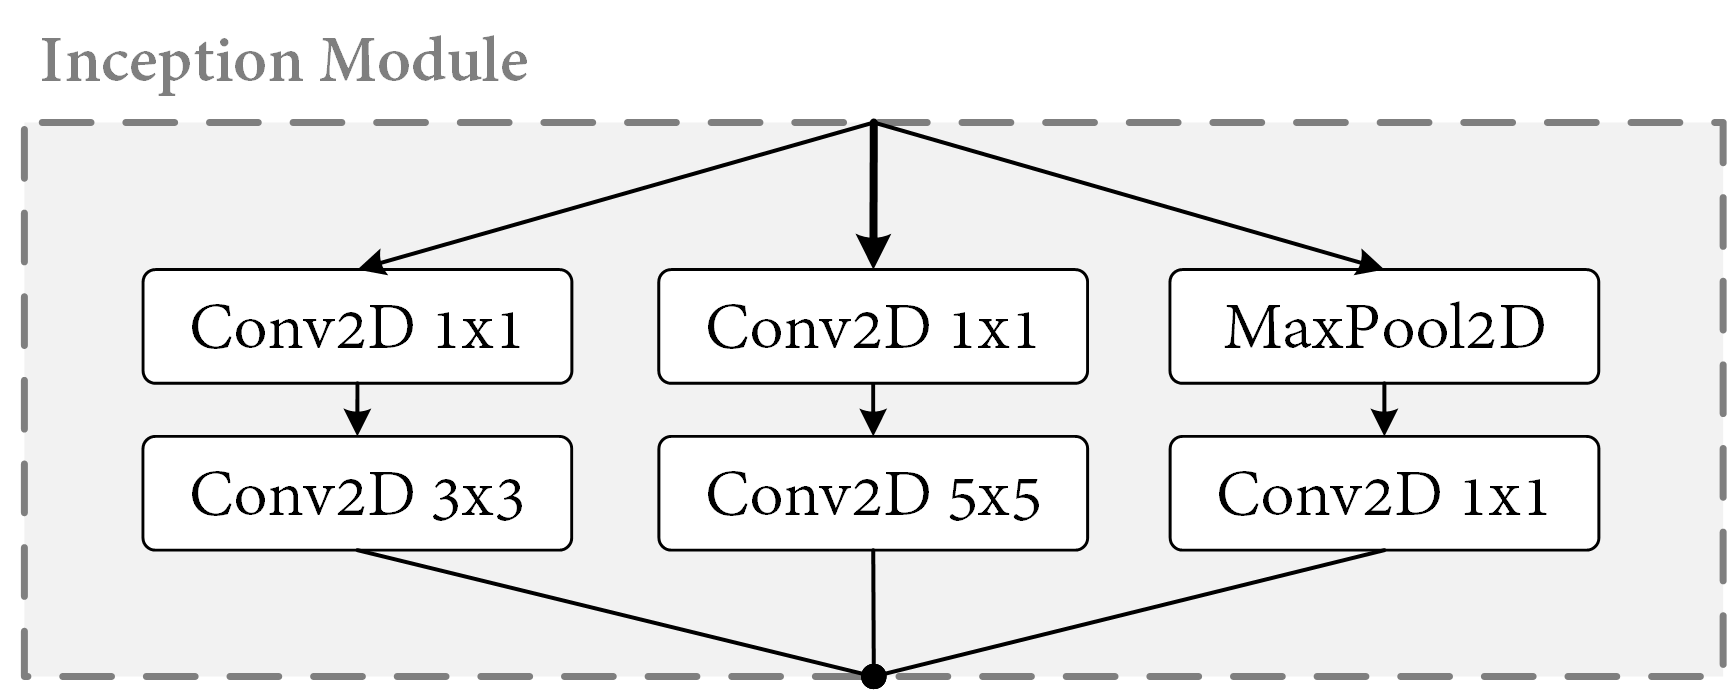
\includegraphics[width=\linewidth]{figs/vineyard_classification/inception_block.png}
	\caption{First proposal of Inception block \cite{szegedy_going_2014}.}
	\label{fig:naive_inception}
\end{marginfigure}
\begin{enumerate}
    \item The first two convolutional layers to extract spectral and spatial features were removed, thus only remaining the two Inception blocks.
    \item Both Inception blocks were modelled using the naïve version, originally proposed by \cite{szegedy_going_2014} (see Figure \ref{fig:naive_inception}). The main difference between this architecture and ours is that the former extracts features with different neighbourhood sizes using the spectral bands as input for the later convolutional layers.
    \item Only the first Inception block was exchanged by a naïve version, as the one used in the previous experiment.
    \item The spatial attention layer was not included.
\end{enumerate}

The obtained results are shown in Table \ref{table:ablation_results}. Removing the SA layers led to a slight decrease in performance, similar to removing the first convolutional layers. However, the latter returned worse results since spectral features were not retrieved prior to normalizing attributes for the first time and passing them to the Inception layers. Unsurprisingly, using the first version of the Inception layer twice led to a significant performance decrease for every metric, as it kept transforming the spectral dimensionality in a deep layer. The second Inception version also transforms spectral features but rather provides them as an additional layer (concatenation) that can be weighted according to their contribution to the output. Following this reasoning, swapping the first Inception layer with the first version of it did not involve a huge performance drop. Improvements to the proposed architecture over the c) variant were very small and therefore may suggest that using either one of them does not offer great changes in the performance. Similar results to this last setup were achieved by removing the spatial attention layer; it did not lead to a significant performance drop, though better results were obtained using it. 

\newcommand{\specialcell}[2][c]{\begin{tabular}[#1]{@{}c@{}}#2\end{tabular}}
\newcommand{\numberVariance}[2]{#1 $\pm$ #2}

\renewcommand{\arraystretch}{1.15}
\begin{table*}
\small
\centering
\caption{Overall results in terms of Overall Accuracy (OA), Average Accuracy (AA) and Kappa coefficient
with different methods.\\ }
\label{table:ablation_results}
\begin{tabular}{|l|*5{c|}}
\toprule
Metric & Ours & \specialcell{1) Without\\ initial convolutions} & \specialcell{2) Double\\ naïve Inception} & \specialcell{3) Naïve \&\\ advanced Inception} & \specialcell{4) Without\\ spatial-attention}\\
\cmidrule{1-6}
\multicolumn{6}{|c|}{\textbf{Red}}\\
\cmidrule{1-6}
OA & \textbf{\numberVariance{99.31}{0.05}} & \numberVariance{98.80}{0.14} & \numberVariance{98.58}{0.08} & \numberVariance{99.00}{0.06} & \numberVariance{99.00}{0.06}\\
AA & \textbf{\numberVariance{99.29}{0.03}} & \numberVariance{98.51}{0.16} & \numberVariance{97.70}{0.13} & \numberVariance{98.98}{0.08} & \numberVariance{98.92}{0.07}\\
Kappa ($\kappa$) & \textbf{\numberVariance{99.20}{0.07}} & \numberVariance{98.21}{0.25} & \numberVariance{98.57}{0.14} & \numberVariance{98.80}{0.08} & \numberVariance{98.86}{0.07}\\
f1 & \textbf{\numberVariance{99.31}{0.05}} & \numberVariance{98.80}{0.14} & \numberVariance{98.58}{0.08} & \numberVariance{99.00}{0.06} & \numberVariance{99.00}{0.06}\\
\cmidrule{1-6}
\multicolumn{6}{|c|}{\textbf{White}}\\
\cmidrule{1-6}
OA & \textbf{\numberVariance{98.43}{0.13}} & \numberVariance{97.87}{0.58} & \numberVariance{97.47}{0.15} & \numberVariance{98.09}{0.16} & \numberVariance{98.14}{0.09}\\
AA & \textbf{\numberVariance{99.18}{0.04}} & \numberVariance{98.81}{0.25} & \numberVariance{98.64}{0.09} & \numberVariance{99.01}{0.09} & \numberVariance{99.01}{0.04}\\
Kappa ($\kappa$) & \textbf{\numberVariance{98.36}{0.16}} & \numberVariance{96.48}{1.16} & \numberVariance{97.24}{0.17} & \numberVariance{97.77}{0.20} & \numberVariance{98.53}{0.04}\\
f1 & \textbf{\numberVariance{98.43}{0.13}} & \numberVariance{97.86}{0.59} & \numberVariance{97.48}{0.15} & \numberVariance{98.09}{0.16} & \numberVariance{98.14}{0.09}\\
\bottomrule
\end{tabular}
\normalsize
\end{table*}
\renewcommand{\arraystretch}{1}

\subsection{Training time and network capacity}

The benchmark on the classification problem is relevant to show that training time is not excessive and that the proposed network does not have much more capacity than the problem warrants. Regarding the capacity, Figure \ref{fig:training_history} shows that training and test signatures are similar, and therefore do not show overfitting nor underfitting behaviours. Furthermore, the training AO and loss worsen as a new dataset is introduced, whereas the validation metrics remain similar. Thus, the network is not memorizing input data. Along with this, the network is only parameterized by nearly 400k parameters, while other state-of-the-art models exceed ten million parameters (see Figure \ref{fig:time_capacity_networks}). The number of parameters is derived from the proposed architectures, using an input of size $23 \times 23 \times 30$. Note that the network of \cite{lu_hyperspectral_2022} was decimated in our experimentation with pooling operations of a lower size than proposed to adapt it to smaller patches. Finally, the response time for training the proposed network is below an hour, whereas others require up to several hours. The fitting over datasets concerning white varieties required half an hour since a faster convergence was achieved and most of the compared network, including ours, exited the training without completing it. Note that every available sample was used during training, instead of using strides; otherwise, the training time can be reduced. Further insight into these results is provided by Table \ref{table:overall_results}.

\renewcommand{\arraystretch}{1.15}
\begin{table*}
\centering
\small
\caption{Overall results in terms of Overall Accuracy (OA), Average Accuracy (AA) and Kappa coefficient
with different methods.\\ }
\label{table:overall_results}
\begin{tabular}{|l|*7{c|}}
\toprule
Metric & Ours & LtCNN & Nezami et al. & JigsawHSI & SpectralNET & HybridSN & A-SPN\\
\cmidrule{1-8}
\multicolumn{8}{|c|}{\textbf{Red variety}}\\
\cmidrule{1-8}
OA & \textbf{\numberVariance{99.31}{0.05}} & \numberVariance{87.37}{2.15} & \numberVariance{92.04}{0.42} & \numberVariance{91.18}{0.78} & \numberVariance{88.57}{0.15} & \numberVariance{69.05}{0.43} & \numberVariance{76.62}{0.63}\\
AA & \textbf{\numberVariance{99.29}{0.03}} & \numberVariance{85.39}{3.02} & \numberVariance{90.94}{0.56} & \numberVariance{91.06}{0.98} & \numberVariance{89.59}{0.26} & \numberVariance{62.51}{0.51} & \numberVariance{70.62}{0.53}\\
Kappa & \textbf{\numberVariance{99.20}{0.07}} & \numberVariance{87.43}{2.24} & \numberVariance{92.87}{0.35} & \numberVariance{90.16}{0.91} & \numberVariance{86.16}{0.25} & \numberVariance{68.96}{0.66} & \numberVariance{76.56}{0.46}\\
f1 & \textbf{\numberVariance{99.31}{0.05}} & \numberVariance{87.65}{2.06} & \numberVariance{92.12}{0.41} & \numberVariance{91.33}{0.76} & \numberVariance{88.66}{0.16} & \numberVariance{70.11}{0.38} & \numberVariance{76.89}{0.52}\\
\cmidrule{1-8}
\multicolumn{8}{|c|}{\textbf{White variety}}\\
\cmidrule{1-8}
OA & \textbf{\numberVariance{98.43}{0.13}} & \numberVariance{79.43}{6.85} & \numberVariance{89.07}{0.87} & \numberVariance{80.42}{5.28} & \numberVariance{71.05}{1.45} & \numberVariance{57.08}{1.25} & \numberVariance{57.53}{1.47}\\
AA & \textbf{\numberVariance{99.18}{0.04}} & \numberVariance{86.47}{6.05} & \numberVariance{92.81}{0.46} & \numberVariance{87.67}{3.59} & \numberVariance{79.41}{1.36} & \numberVariance{69.52}{1.08} & \numberVariance{72.58}{1.14}\\
Kappa & \textbf{\numberVariance{98.36}{0.16}} & \numberVariance{77.17}{8.01} & \numberVariance{85.84}{1.07} & \numberVariance{80.51}{4.26} & \numberVariance{72.15}{1.30} & \numberVariance{50.44}{1.6} & \numberVariance{49.91}{3.03}\\
f1 & \textbf{\numberVariance{98.43}{0.13}} & \numberVariance{79.20}{7.08} & \numberVariance{88.99}{0.91} & \numberVariance{80.35}{5.00} & \numberVariance{70.87}{1.45} & \numberVariance{56.01}{1.37} & \numberVariance{55.37}{2.03}\\
\bottomrule
\end{tabular}
\normalsize
\end{table*}
\renewcommand{\arraystretch}{1}

\begin{figure*}[ht]
    \centering
    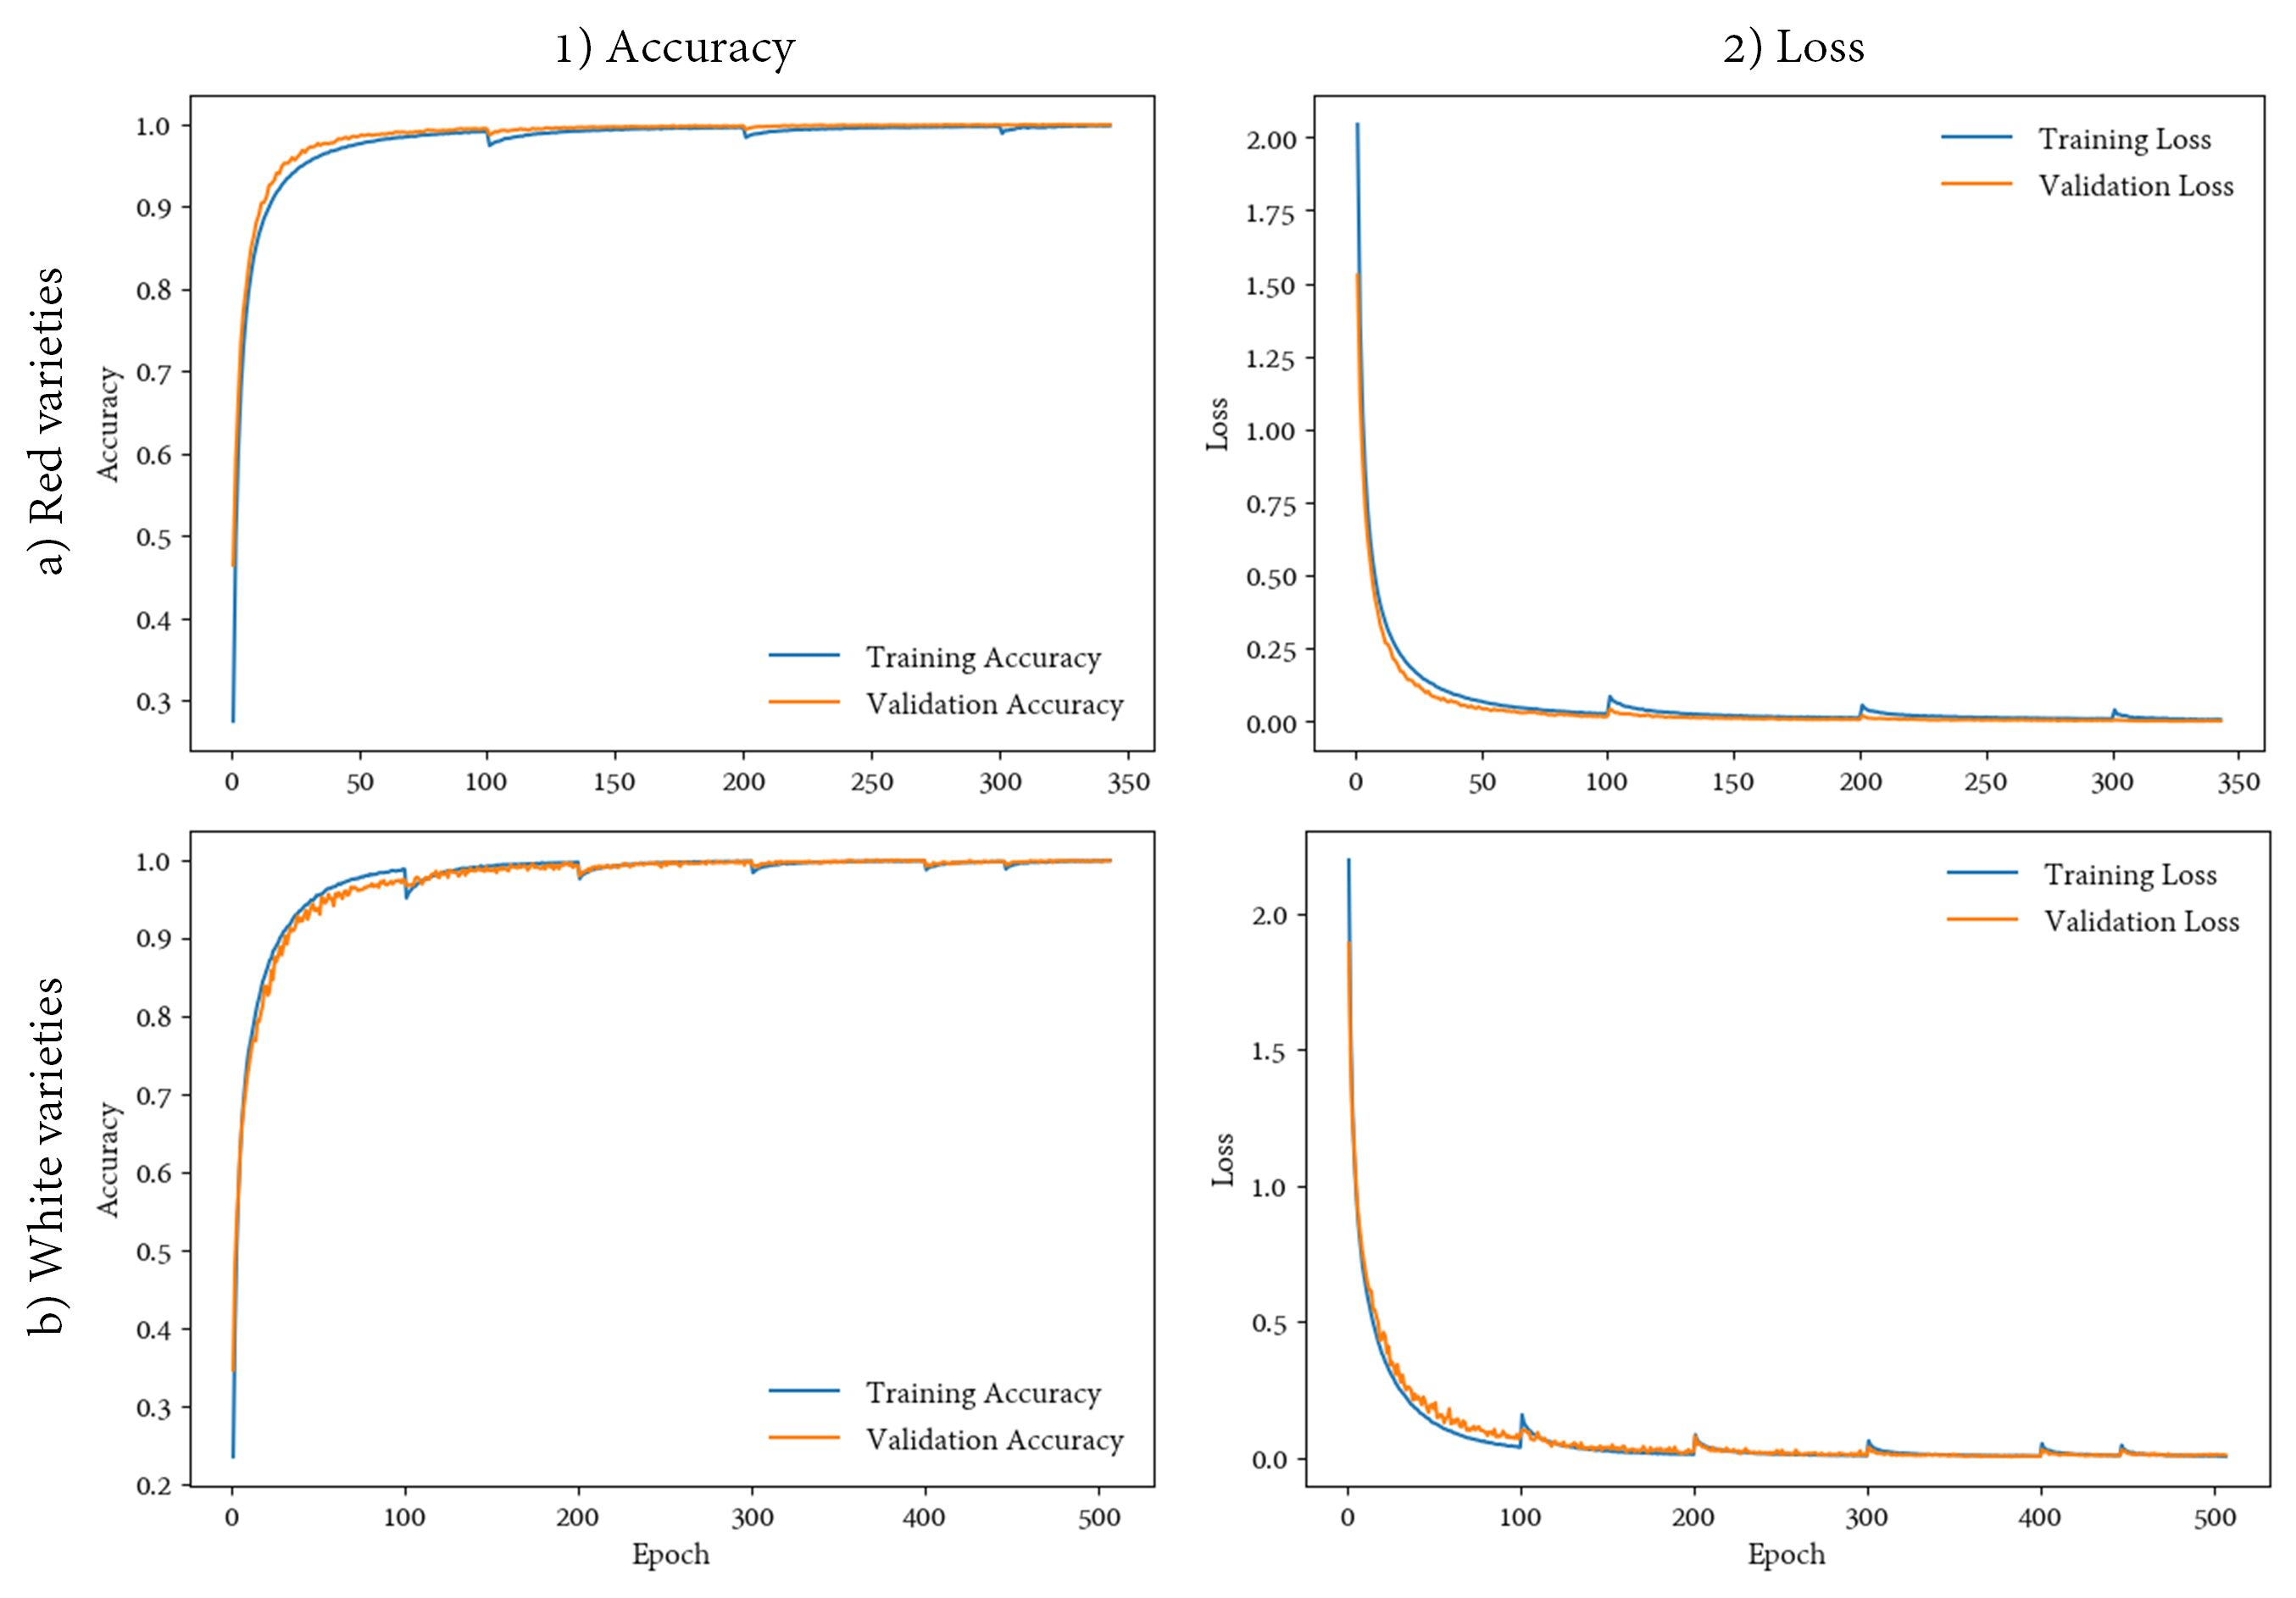
\includegraphics[width=.9\linewidth]{figs/vineyard_classification/training_history.png}
	\caption{Overall accuracy and loss during training. }
	\label{fig:training_history}
\end{figure*}

\begin{figure*}[ht]
    \centering
    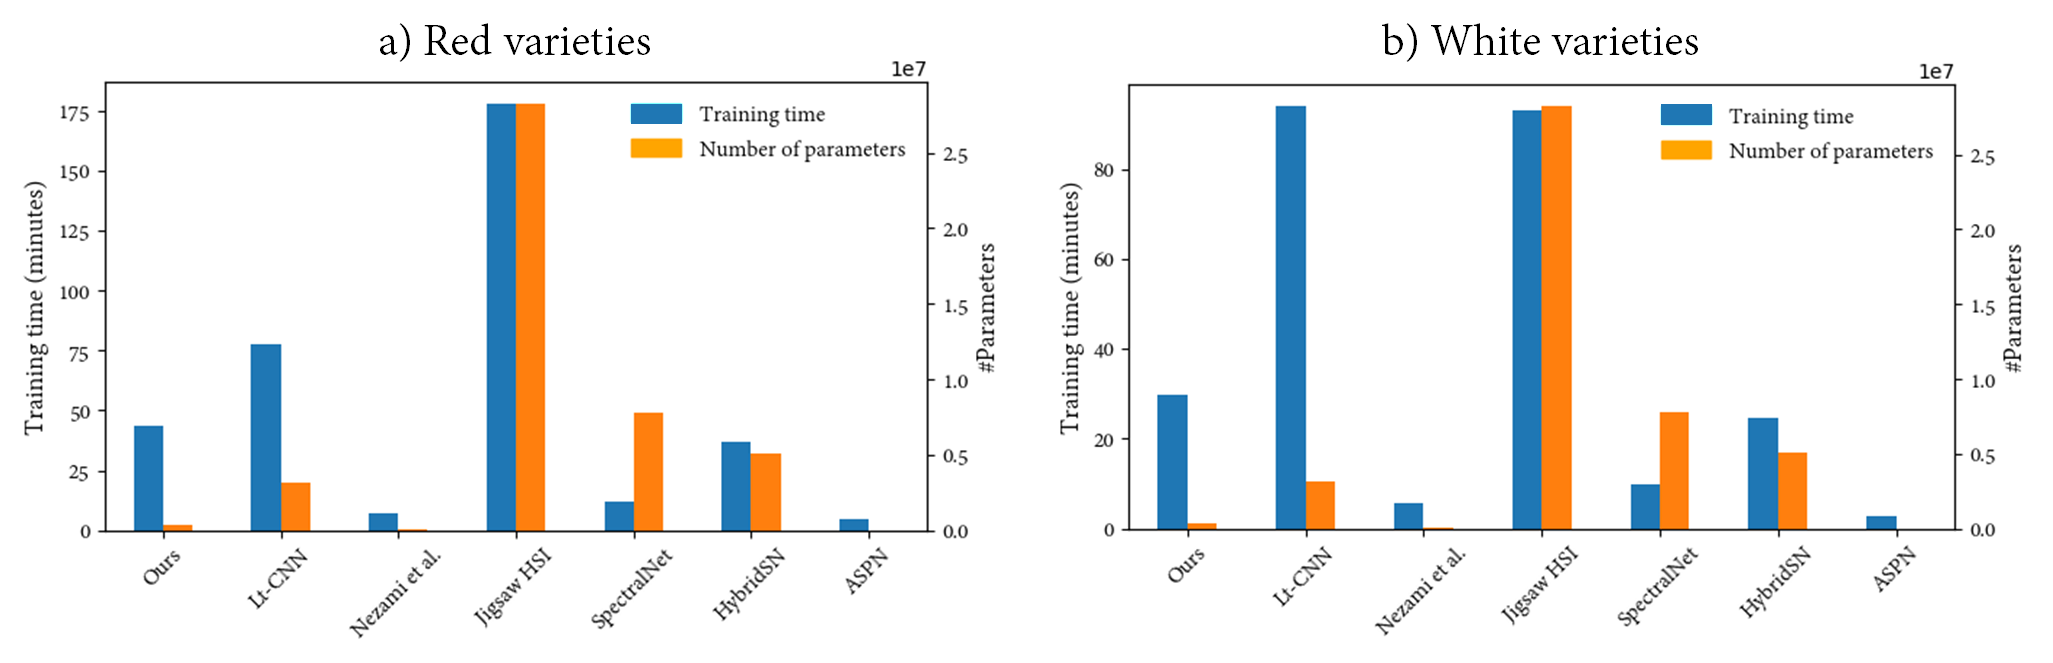
\includegraphics[width=.85\linewidth]{figs/vineyard_classification/time_capacity_network.png}
	\caption{Response time for training the network over a) red and b) white grapevine samples, as well as the number of parameters for every compared network, including ours.  }
	\label{fig:time_capacity_networks}
\end{figure*}

\subsection{Separability}

\begin{marginfigure}[.1cm]
    \centering
    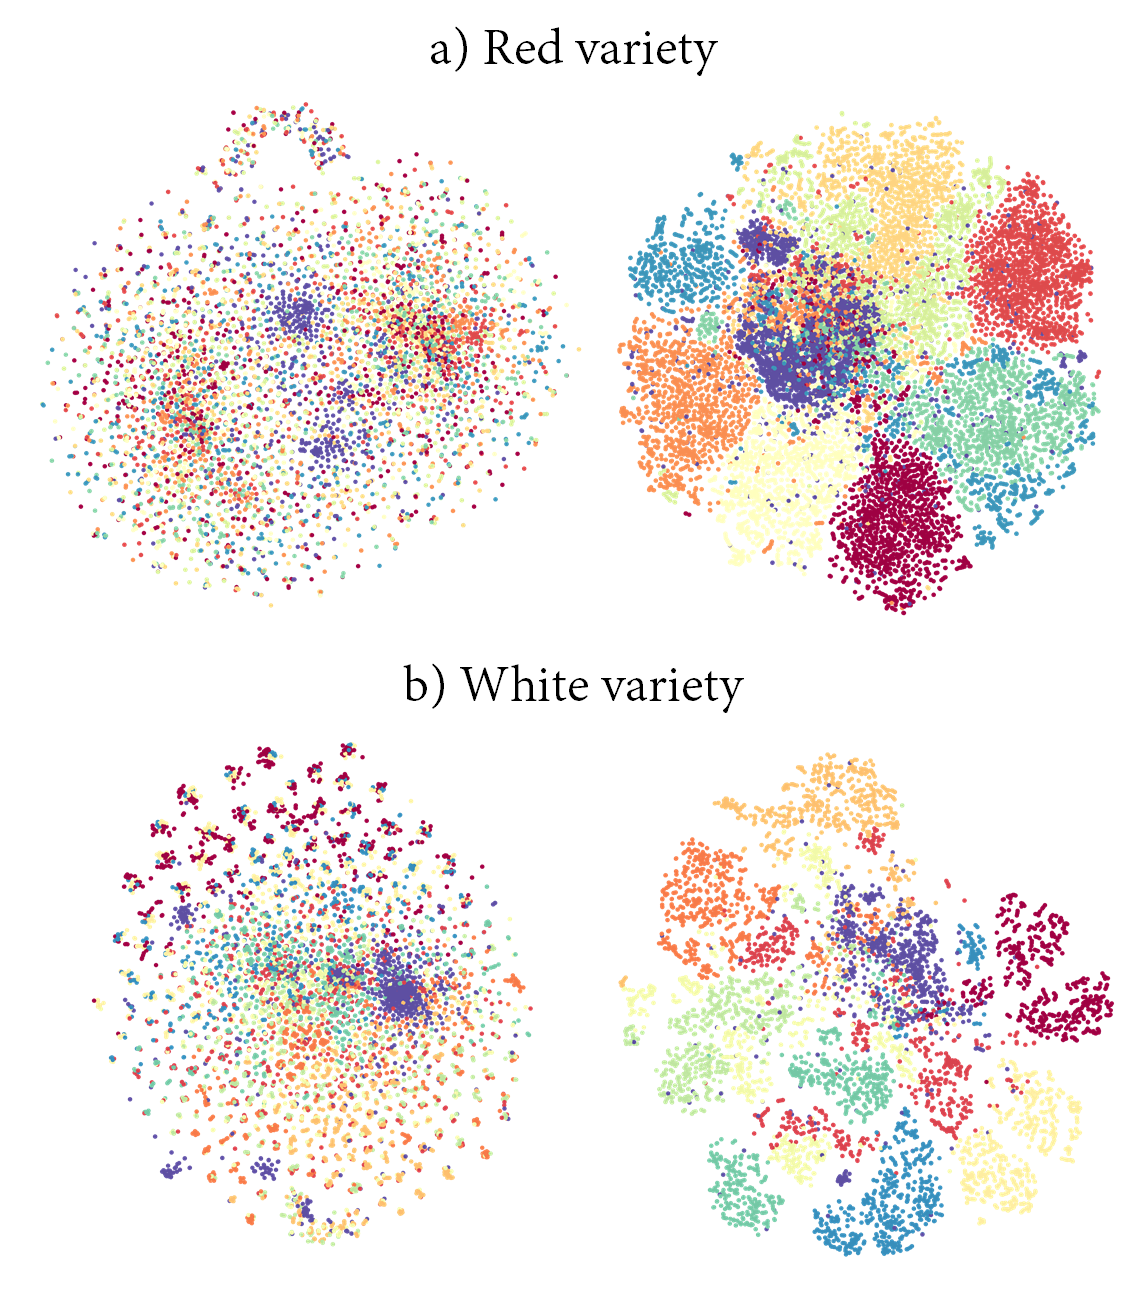
\includegraphics[width=\linewidth]{figs/vineyard_classification/separability.png}
	\caption{Clustering of samples according to the feature transformation performed by uMAP over 1) the starting hyperspectral features and 2) features extracted by the CNN prior to transferring it to the final Softmax layer. }
	\label{fig:separability_umap}
\end{marginfigure}
The output of the proposed network can be assessed in terms of separability by removing the final Dropout and Dense layers. Data is transformed and flattened according to the network's learnt weights. It is subsequently embedded with uMAP \cite{mcinnes_umap_2020} to compress high-dimensionality data into a few features, thus allowing us to visualize the new data representation. The same procedure can be followed over the original data to compare how was the data manifold uncrumpled. As shown in Figure \ref{fig:separability_umap}, different labels were not perfectly unmixed, although the improvement in comparison to the starting representation is notable. To provide this result, the last Flatten layer was connected to uMAP fitting with $n = 2$; hence, 2592 features were narrowed to two features to represent the embedding in a two-dimensional chart.

\subsection{Confusion matrices}

Figure \ref{fig:confusion_matrices} shows the OA of the proposed network against any grape variety. Hence, classification over red varieties showed uniform results, with most of them being close to 99\%. Note that these percentages were rounded, and therefore, some of these results are below 99\%, while others are above. When averaged, all these results lead to an OA of $\approx99.3$\%, as shown in Table \ref{table:overall_results}. On the other hand, most white varieties were better classified, with a significant number being perfectly annotated. However, others were more often mistaken, for instance, class five, which led to a worse OA.  

\begin{figure*}[ht]
    \centering
    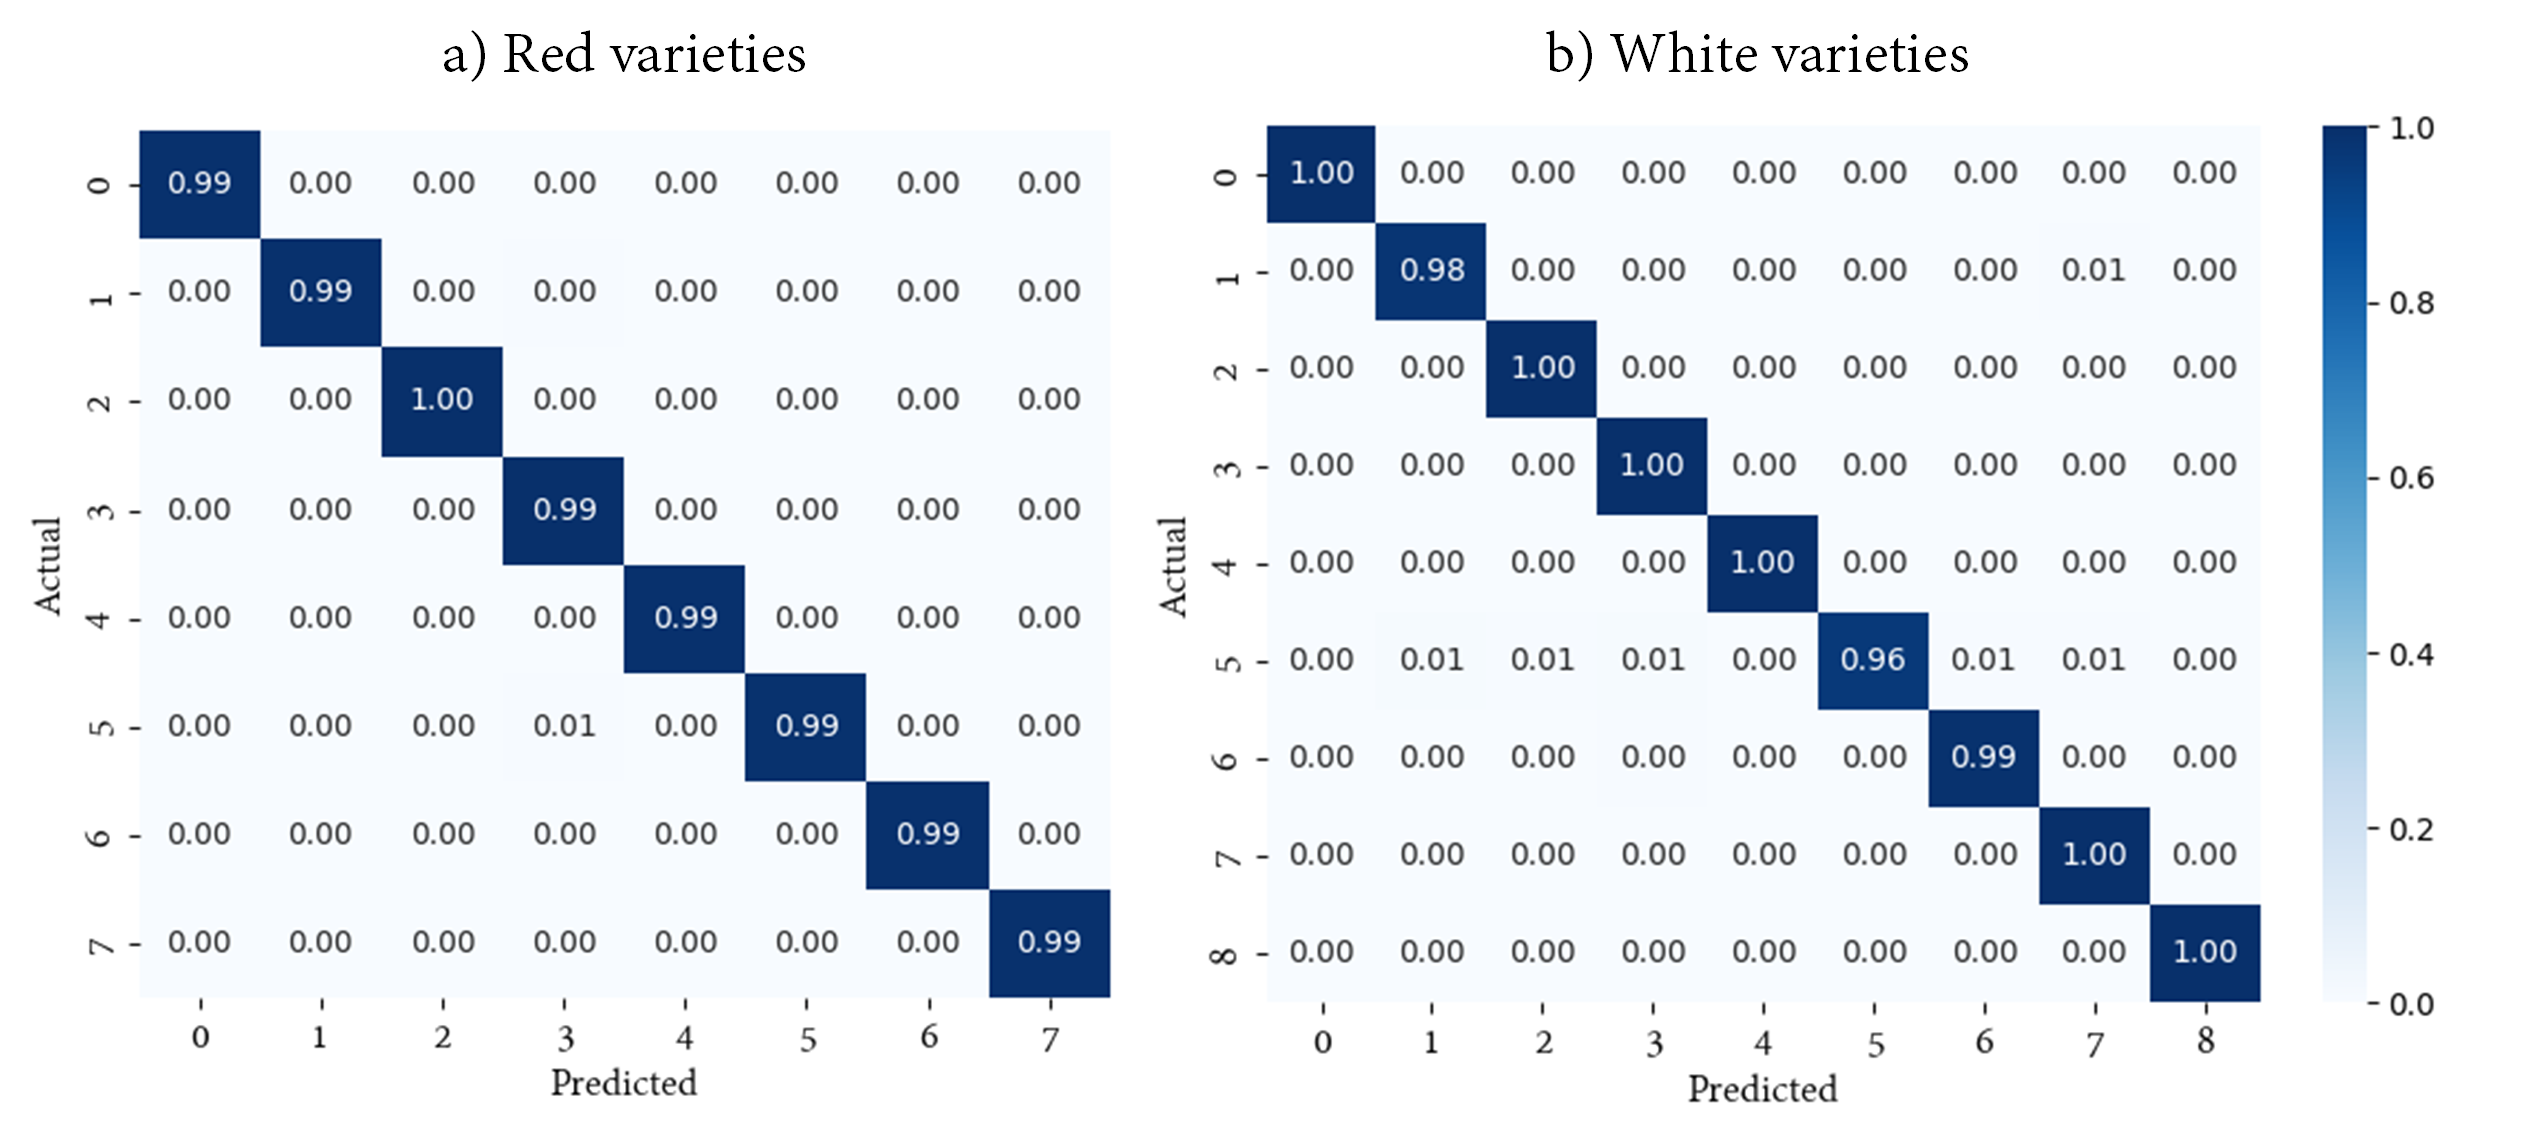
\includegraphics[width=\linewidth]{figs/vineyard_classification/confusion_matrices.png}
	\caption{Confusion matrices for the classification of red and white varieties. }
	\label{fig:confusion_matrices}
\end{figure*} 

\subsection{Analysis of errors}

As observed in previous sections, our architecture achieved a high OA and AA. Still, there is a margin for improvement that must be tackled by finding which are the weaknesses in the overall labelling, transformation and classification pipeline. Instead of predicting randomly selected samples, another experiment is to predict every hyperspectral swath sample, thus allowing us to determine where errors take place within the study area. As observed in Figure \ref{fig:spatial_labelling_errors}, these errors are spatially clustered instead of being sparsed over the study area. If these are compared against the RGB mosaic of the hypercubes, errors are observed to belong to 1) small vegetation clusters, mainly proceeding from small vegetation mistakenly labelled as vineyard and 2) samples surrounded by ground or metallic vineyard supports. Note that these are hard to notice during the labelling since they present signatures similar to the target leaves and they are surrounded by vegetation, thus hardening the definition of a geometrical shape for rapidly tagging which is relevant or not. Still, some errors are present in grape samples surrounded by ground and other surfaces since these have a notable impact on the sample's neighbourhood, thus distorting the final probability. Note that every boundary sample is surrounded by vegetation, and therefore, it should be expected that their signature is the fusion of the signatures concerning a target variety and ground. However, it may be not relevant enough to tell apart varieties, thereby leading to more errors on samples heavily surrounded by ground.

\begin{figure}[ht]
    \centering
    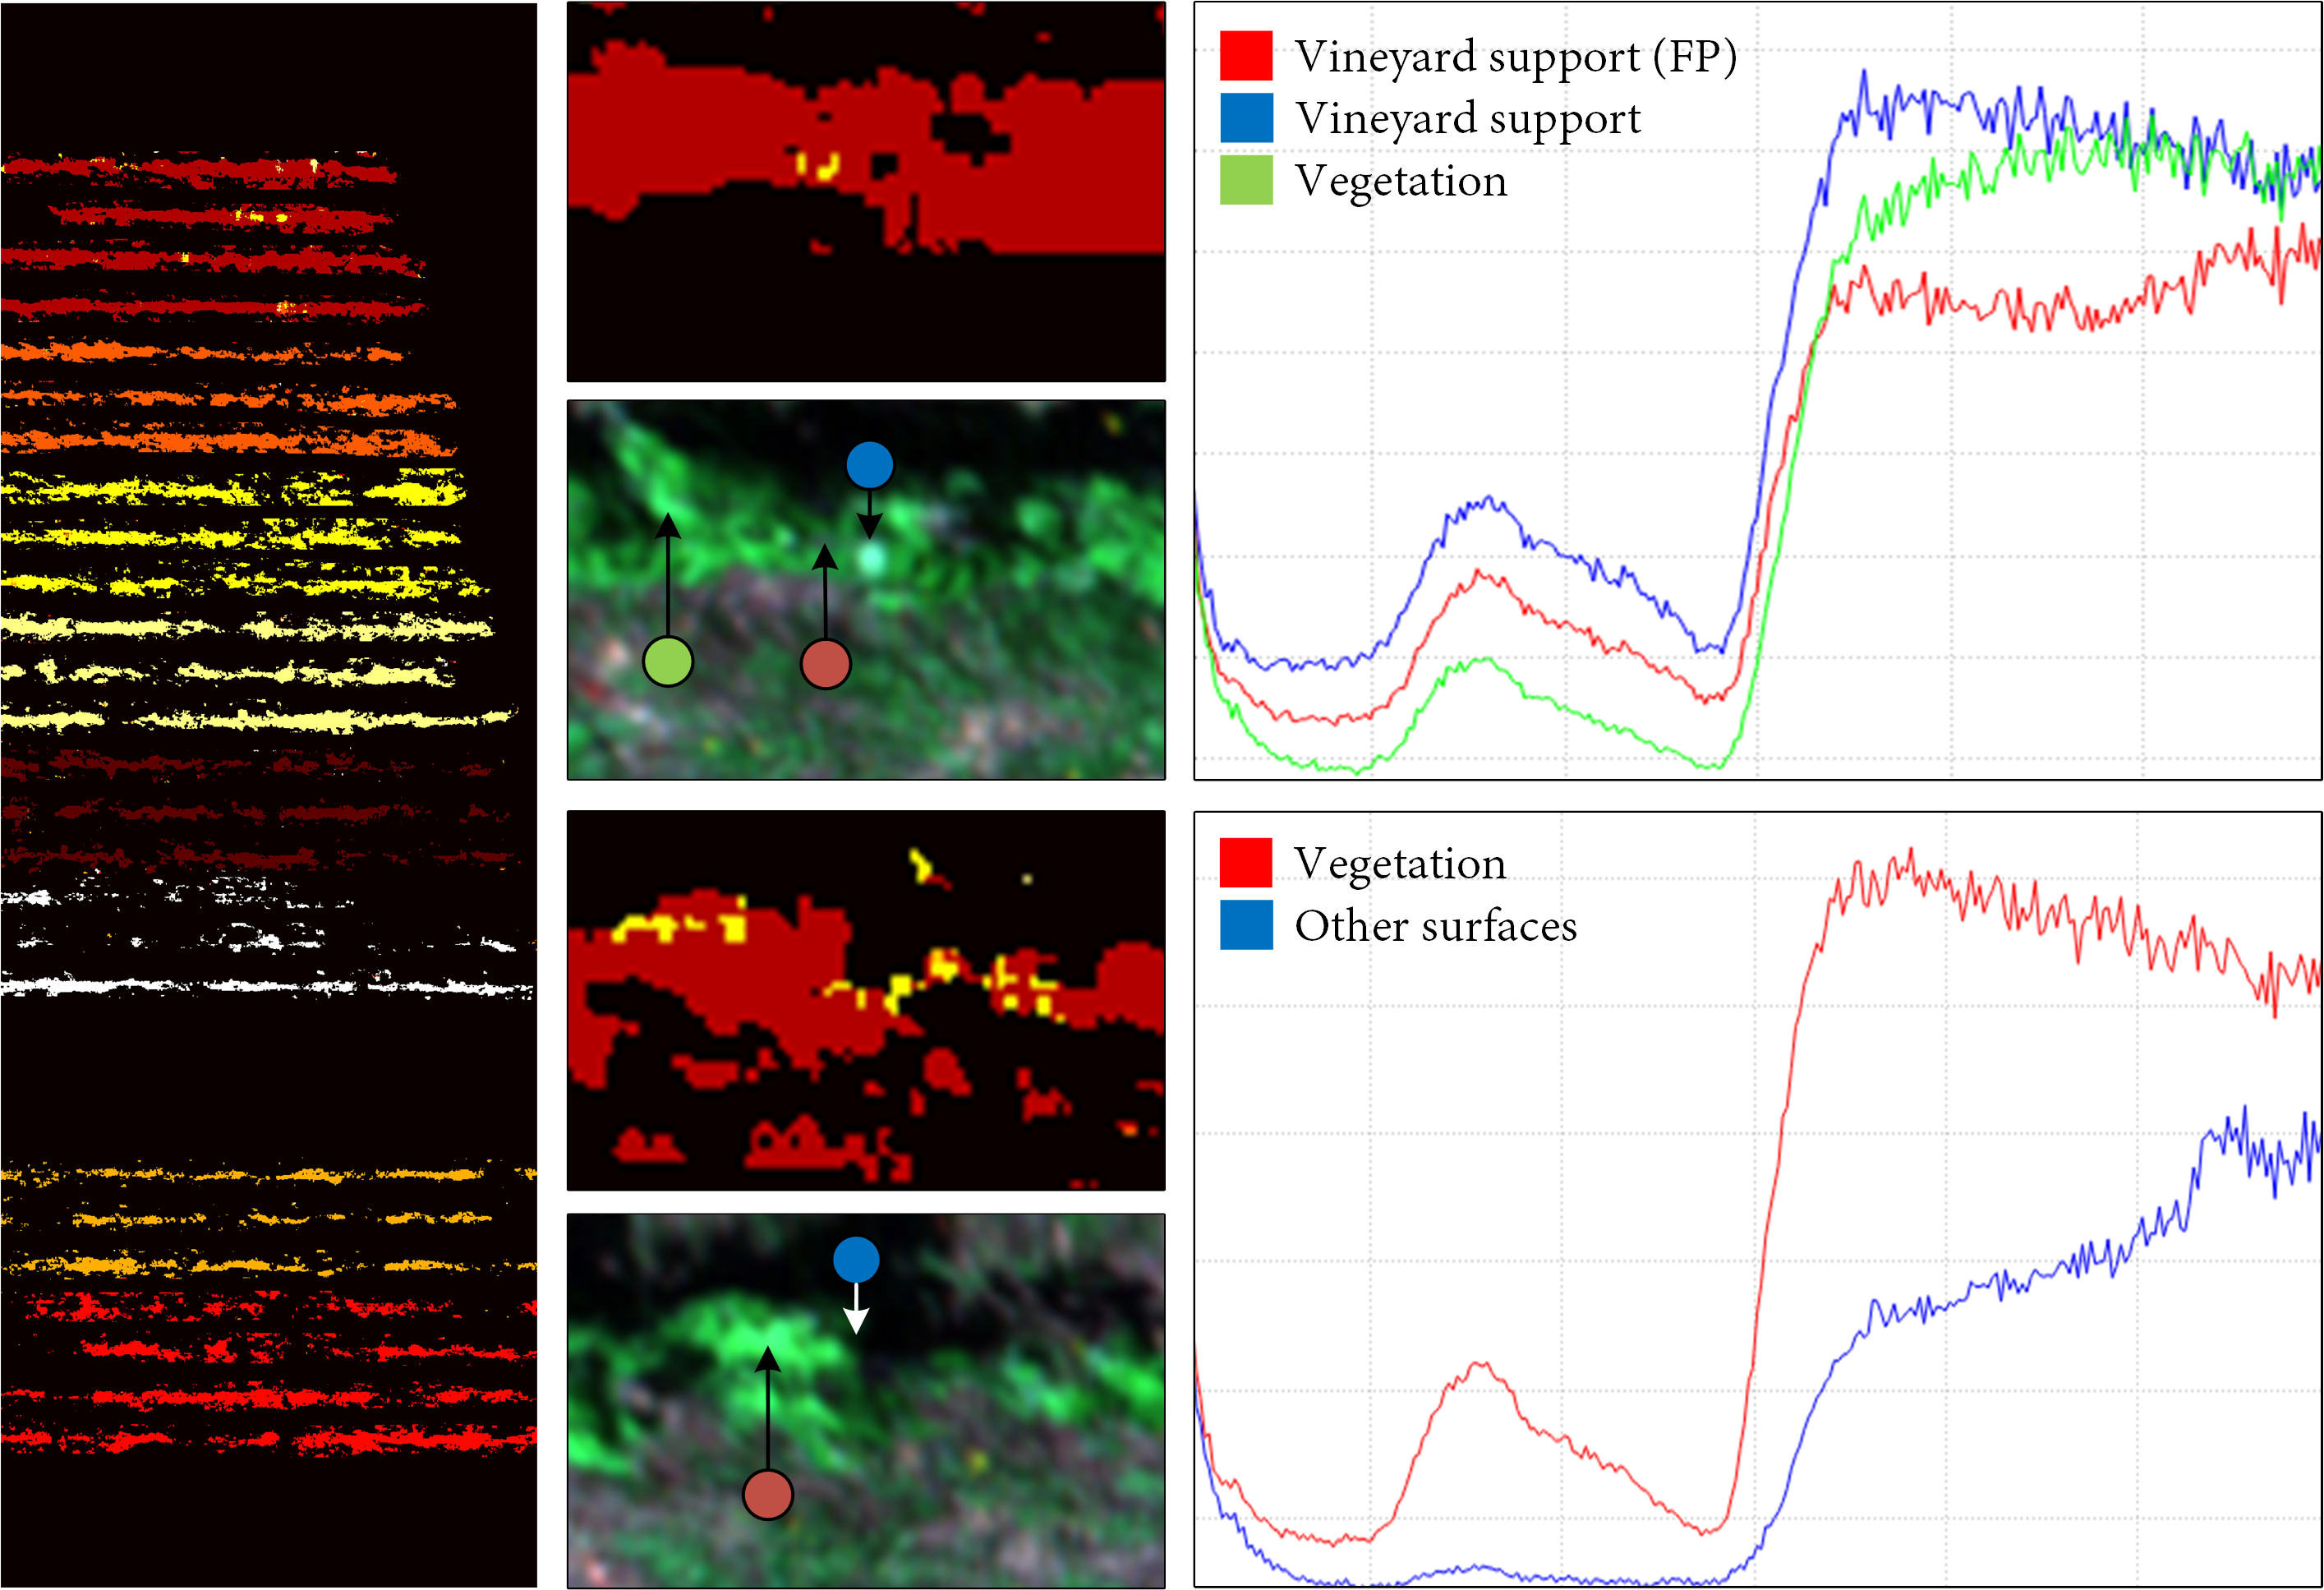
\includegraphics[width=\linewidth]{figs/vineyard_classification/spatial_labelling.png}
	\caption{Errors observed in the classification of red varieties, together with the hyperspectral signature of a few samples concerning different surfaces.  }
	\label{fig:spatial_labelling_errors}
\end{figure}

\subsection{Training over satellite imagery}

The main shortcoming of compared CNNs focused on satellite imagery is that they obtain a poor performance over the proposed UAV datasets and vineyard varieties. Hyperspectral imagery from UAVs is noisier than satellite observations, with the spectral signature of the latter being more smoothed out. Therefore, previous work did not overcome noise in the classification of vineyards and most of them showed poor performance. Only another architecture tested over UAV samples managed to reach an OA near 90\%, whereas others showing similar results proposed huge networks with millions of parameters, thus overkilling the classification with a large training time. 

The aim of this chapter is to remark on how our network behaves over satellite hyperspectral imagery. Although the network was not designed for this purpose, several tests were launched over publicly available datasets frequently used for comparison. The number of labels in these data ranges from nine to sixteen, and the number of spectral bands also differs from our imaging device. However, FA was fitted to obtain only 30 features per pixel, as proposed for UAV imagery, and so does the architecture of the network. According to the number of samples of each dataset, the batch size was adapted as shown in Table \ref{table:satellite_results}. Every dataset had unlabelled samples which were removed from the training and test datasets to establish a fair comparison with previous work. Unlike our UAV datasets, labels in satellite imagery were imbalanced, with some of them having only a few dozen of examples. Hence, balancing was not applied in satellite datasets to avoid levelling the rest of the classes with others that present scarce examples. 

From the results, it can be observed that the proposed network can also be applied to this kind of imagery despite not being its main area of expertise. All of the datasets converged early to classification metrics over 98\%, and despite not providing state-of-the-art results, these are very close to the current networks that show the best performance. As we did not intend to tune the network for satellite imagery, the learning rate remained as before, and the batch size was scaled according to the number of samples.

\renewcommand{\arraystretch}{1.1}
\begin{table*}
\small
\centering
\caption{Classification of hyperspectral imagery from satellite platforms in terms of Overall Accuracy (OA) and Kappa coefficient ($\kappa$).\\ }
\label{table:satellite_results}
\begin{tabular}{|l@{}|*6{c|}}
\toprule
& \multicolumn{3}{c|}{Ours} & \multicolumn{3}{c|}{State-of-the-art}\\
\cmidrule{1-7}
Dataset & OA & Kappa ($\kappa$) & Batch size & OA & Kappa ($\kappa$) & Reference work \\
\cmidrule{1-7}
\textbf{Pavia university} & \numberVariance{99.77}{0.02} & \numberVariance{99.70}{0.06} & 128 & \numberVariance{100}{0.00} & \numberVariance{100}{0.00} & \cite{moraga_jigsawhsi_2022}\\
\cmidrule{1-7}
\textbf{Indian pines} & \numberVariance{99.92}{0.00} & \numberVariance{99.96}{0.00} & 128 & \numberVariance{99.93}{0.07} & \numberVariance{99.89}{0.10} & \cite{ravikumar_hyperspectral_2022}\\
\cmidrule{1-7}
\textbf{Salinas valley} & \numberVariance{100}{0.00} & \numberVariance{100.0}{0.00} & 512 & \numberVariance{100}{0.00} & \numberVariance{100}{0.00} & \cite{moraga_jigsawhsi_2022}\\
\bottomrule
\end{tabular}
\normalsize
\end{table*}
\renewcommand{\arraystretch}{1}

\section{Conclusions and future work}

The proposed network presents a CNN model that uses current state-of-the-art procedures applied to classify grapevine varieties. Spatial-attention layers were proved to enhance the results, whereas Inception layers were checked to discuss which one could provide better results over hyperspectral imagery. Note that the majority of CNN works in the literature are oriented towards RGB imagery, and therefore, their transition to hypercubes is not as trivial. Also, only a few works have addressed the classification of UAV-based HSI, since it is considerably noisier. Despite this network being proposed for phenotyping applied to grapevines, it was also tested over standard satellite HSI datasets which are frequently used to establish fair comparisons. The results showed that samples from satellite imagery were also classified with notable accuracy (over 99.7\%), although current state-of-the-art networks achieve better results. In contrast, most of the compared models achieved poor results over UAV-based imagery ($\sim90$\% at most). Our training time and the number of parameters were also lower than most of the compared classification models; some of them are composed of millions of parameters, whereas ours solely consist of $\sim400K$ parameters. 

Another explored step, which may be the most relevant, is the preprocessing of reflectance. First, hypercubes are composed of a huge number of bands that cannot be processed by CNNs in a reasonable response time. Furthermore, it hardens the fitting stage and most of these bands may be either redundant or irrelevant to the classification. A significant number of feature reduction and transformation methods were checked, which led to Factor Analysis as the one providing better results in an automatic pipeline. The latter concept is relevant since other methods may be capable of providing better clusters at the expense of demanding the number of different materials collected in hyperspectral imagery. Using FA, hypercubes with 270 bands were narrowed to only 30 features which led to reducing the number of trained parameters and response time. 

Regardless of the high OA and AA, the analysis of errors also depicted some clustered samples that were mislabelled. If checked against false-colour RGB imagery from hypercubes, most of them were low-vegetation labelled as grape varieties, or samples surrounded by other surfaces which hardened the classification. 

As a future work, we would like to further extend this network to integrate as many more varieties as possible. It also ought to be explored whether a different growth stage has some effects on the classification. Hence, proving this would enable this work to be used over any study area at any stage of the year as long as it comprises some of the varieties over which the model has been trained. Also, a considerable effort is being made to collect information about crops receiving grants from national and European funds. For instance, it should be inferred whether a crop is abandoned or not to make a decision on whether these funds are granted. Similarly to this, estimating the area of vineyard rows, even the harvested varieties, could also help in this and other decision-making processes. Finally, the labelling may greatly benefit from using the Digital Elevation Model as collected by the surveying UAV, in order to avoid some labelling errors and speed up this manual task. 

\section*{Additional material}

\newcommand{\varietySpacing}{\hskip 0.25in}
\renewcommand{\arraystretch}{1.1}
\begin{table*}[bp]
\centering
\caption{Summary of information collected from different grapevine varieties. For each variety, the number of field rows is shown, along with the number of laboratory samples and the number of collected leaves. Regarding UAV acquisition, samples are obtained by labelling aerial imagery.\\ }
\label{table:grape_samples}

\begin{tabular}{|*6{l@{\varietySpacing}|}}
\cmidrule{4-6}
\multicolumn{2}{c}{} & & \multicolumn{2}{|c|}{Spectrometer} & \multicolumn{1}{c|}{UAV}\\
\cmidrule{1-6}
\textbf{Root variety} & \textbf{Variety} & \textbf{\#Rows} & \textbf{\#Leaves} & \textbf{\#Samples} & \textbf{\#Samples}\\
\cmidrule{1-6}
\multirow{9}{*}{Red} & Alicante & 3 & 8 & 96 & 20,910\\
& Alvarhelao & 4 & 6 & 36 & 100,285\\
& Barroca & 3 & 9 & 108 & 17,219\\
& Sousao & 3 & 6 & 36 & 29,960\\
& Touriga Femea & 3 & 6 & 36 & 38,568\\
& Touriga Francesa & 3 & 9 & 54 & 14,894\\
& Touriga National & 3 & 9 & 108 & 38,925\\
& Tinta Roriz & 4 & 9 & 108 & 31,091\\
\cmidrule{1-6}
\multirow{9}{*}{White} & Arito Do Douro & 1 & 6 & 50 & 58.813\\
& Boal & 3 & 8 & 72 & 22,751\\
& Cercial & 1 & 6 & 36 & 13,556\\
& Codega Do Ladinho & 3 & 16 & 140 & 146,083\\
& Donzelinho Branco & 1 & 2 & 12 & 34,019\\
%& Falgasao & 1 & 6 & 36 & 13,539\\
& Malvasia Fina & 3 & 16 & 129 & 139,985\\
& Moscatel Galego & 1 & 6 & 54 & 48,352\\
& Moscatel Galego Roxo & 1 & 6 & 36 & 47,745\\
& Samarrinho & 1 & 6 & 36 & 43.560\\
\bottomrule
\end{tabular}
\end{table*}
\renewcommand{\arraystretch}{1}

\begin{figure*}[bp]
    \centering
    {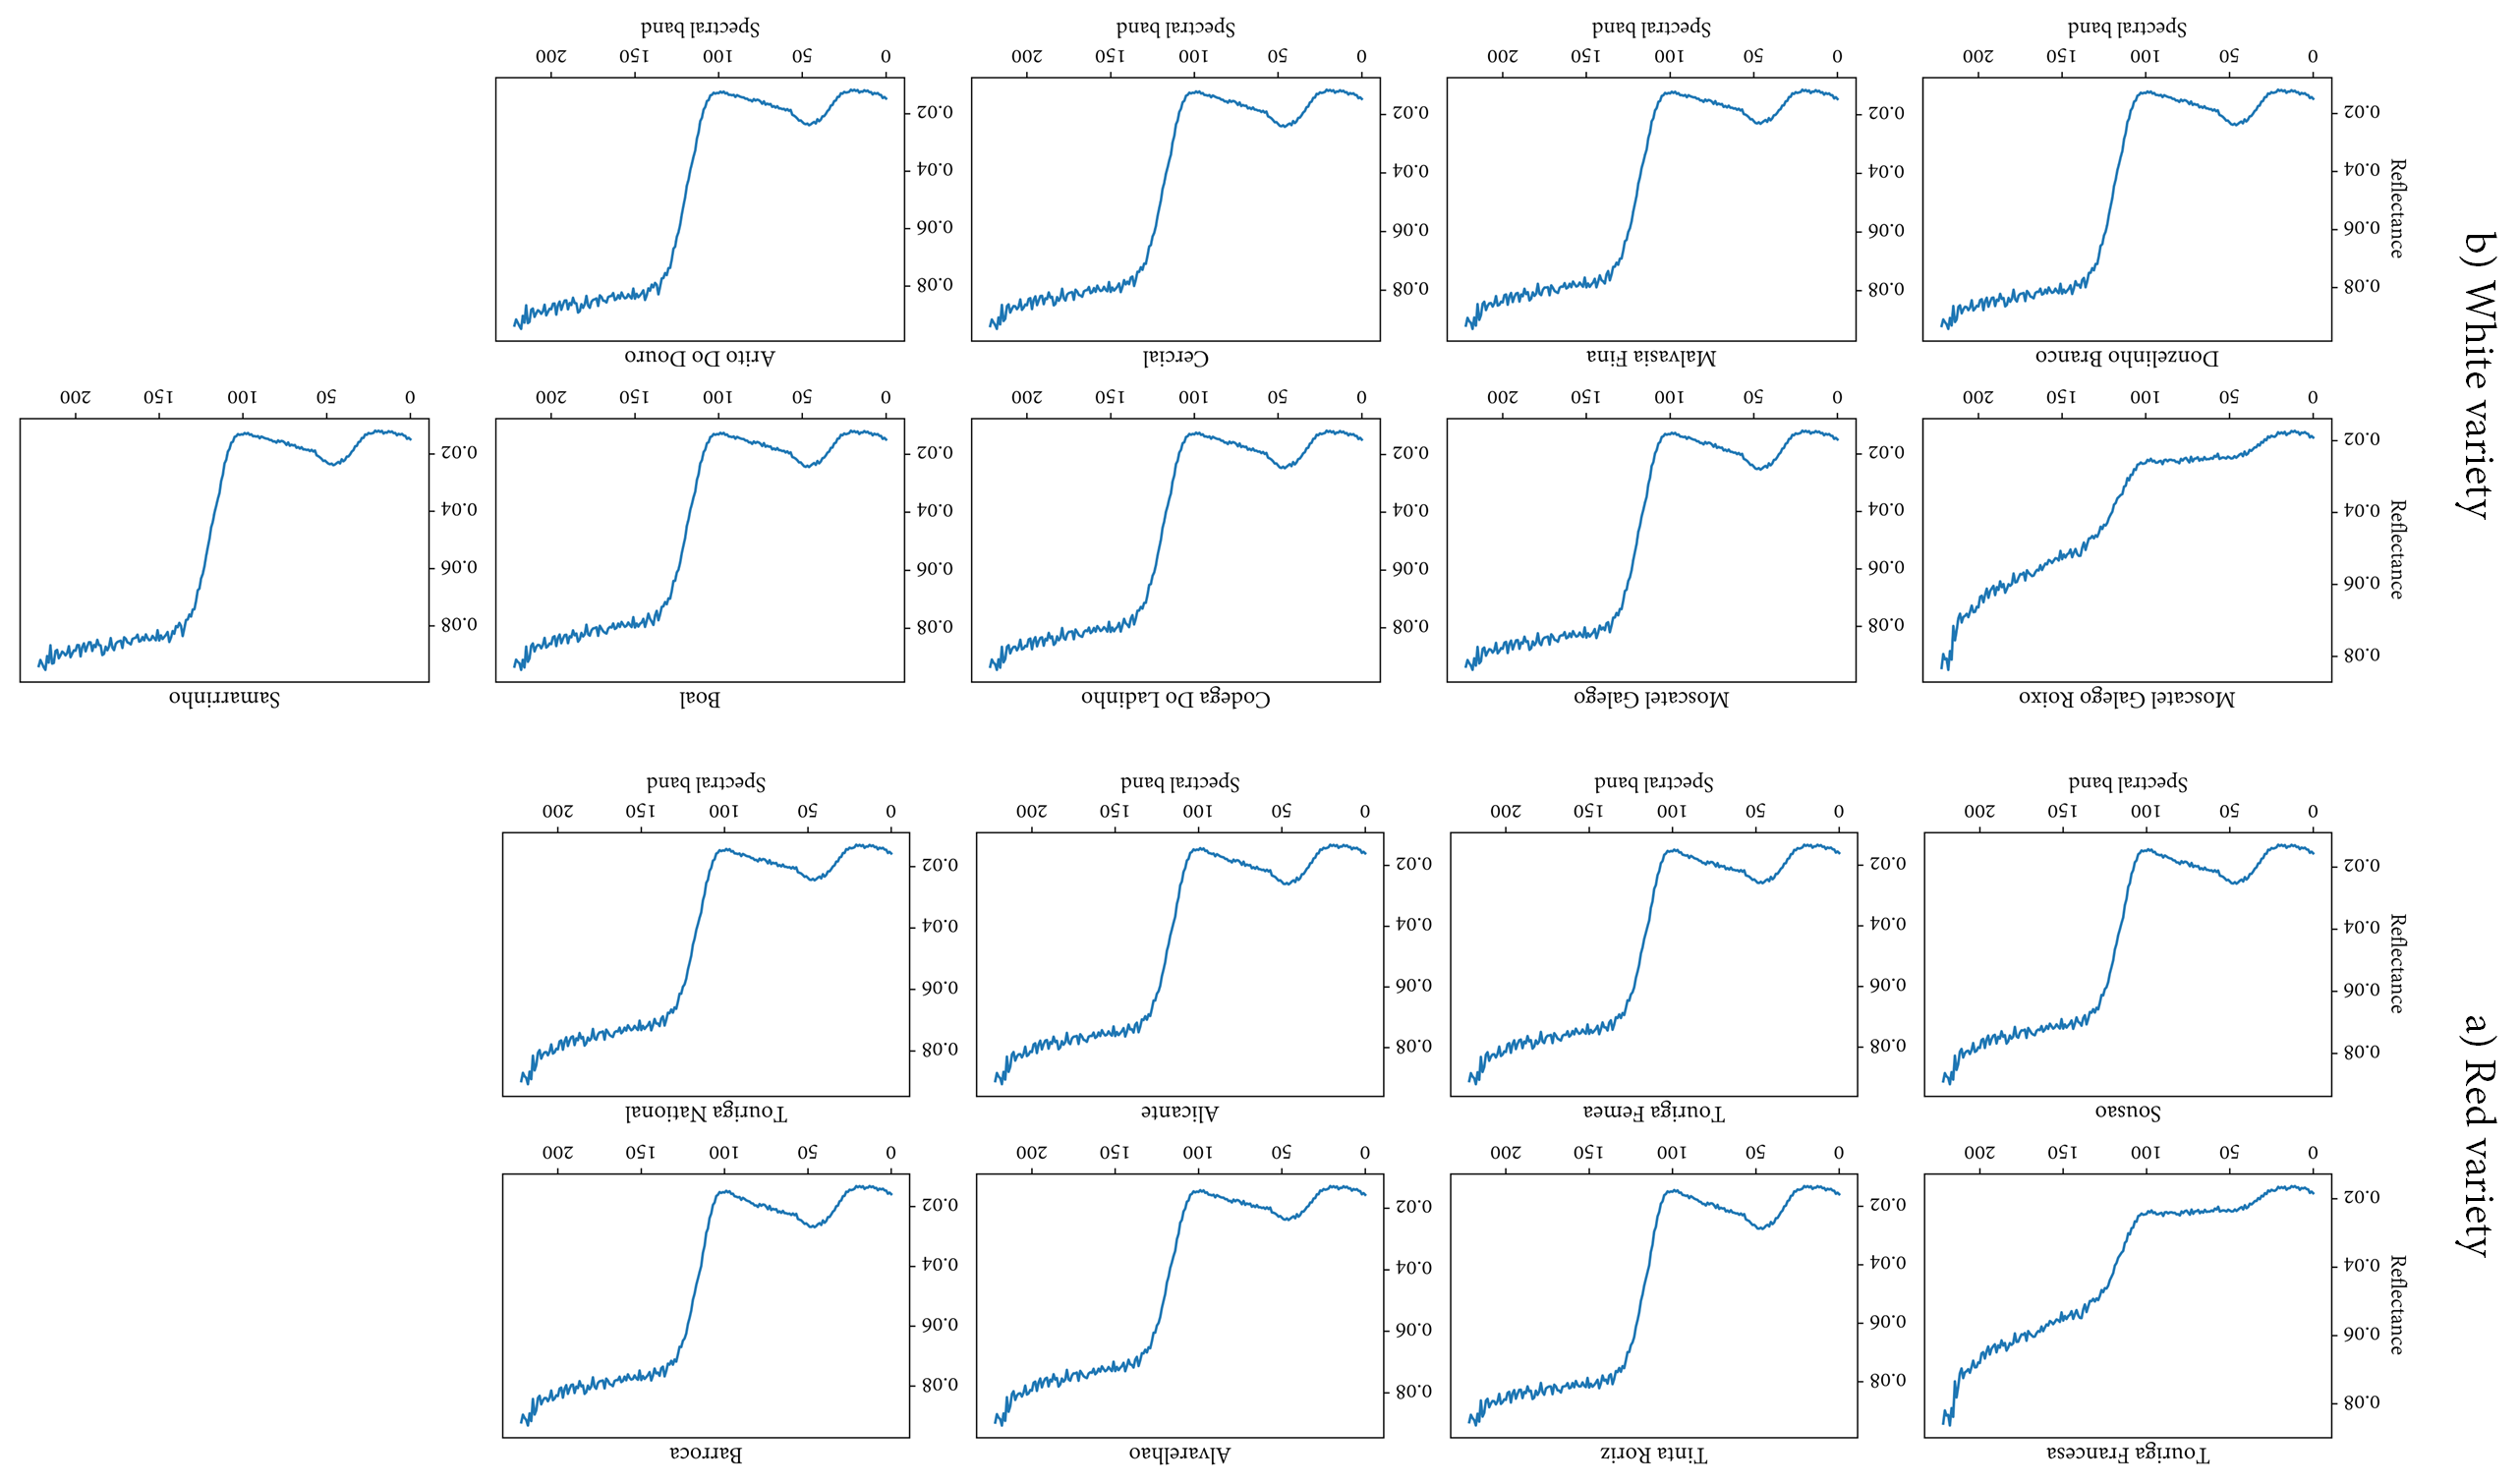
\includegraphics[width=\linewidth]{figs/vineyard_classification/vineyard_signature_grid.png}}
	\caption{Mean spectral signature of a) red and b) white grape varieties. }
	\label{fig:vineyard_mean_grid}
\end{figure*}

\begin{figure*}[bp]
    \centering
    {\includegraphics[width=\linewidth]{figs/vineyard_classification/swaths.png}}
	\caption{False RGB color images from the collected hypercubes depicting two different areas, focused on 1) red and 2) white grapevine varieties.}
	\label{fig:vineyard_swaths}
\end{figure*}

\begin{figure}[ht]
    \centering
    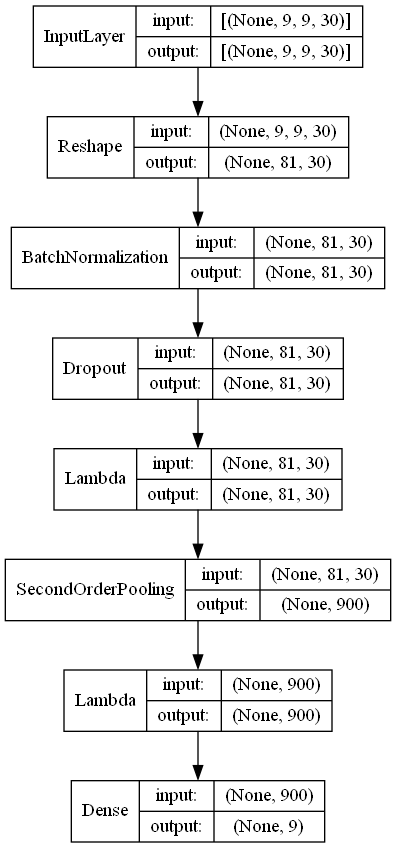
\includegraphics[width=.7\linewidth]{figs/vineyard_classification/networks/aspn_9x8_32.png}
	\caption{CNN architecture proposed by Xue et al. \cite{xue_attention-based_2021} as implemented in this study to establish a comparison. }
	\label{fig:aspn_cnn}
\end{figure}

\begin{figure}[ht]
    \centering
    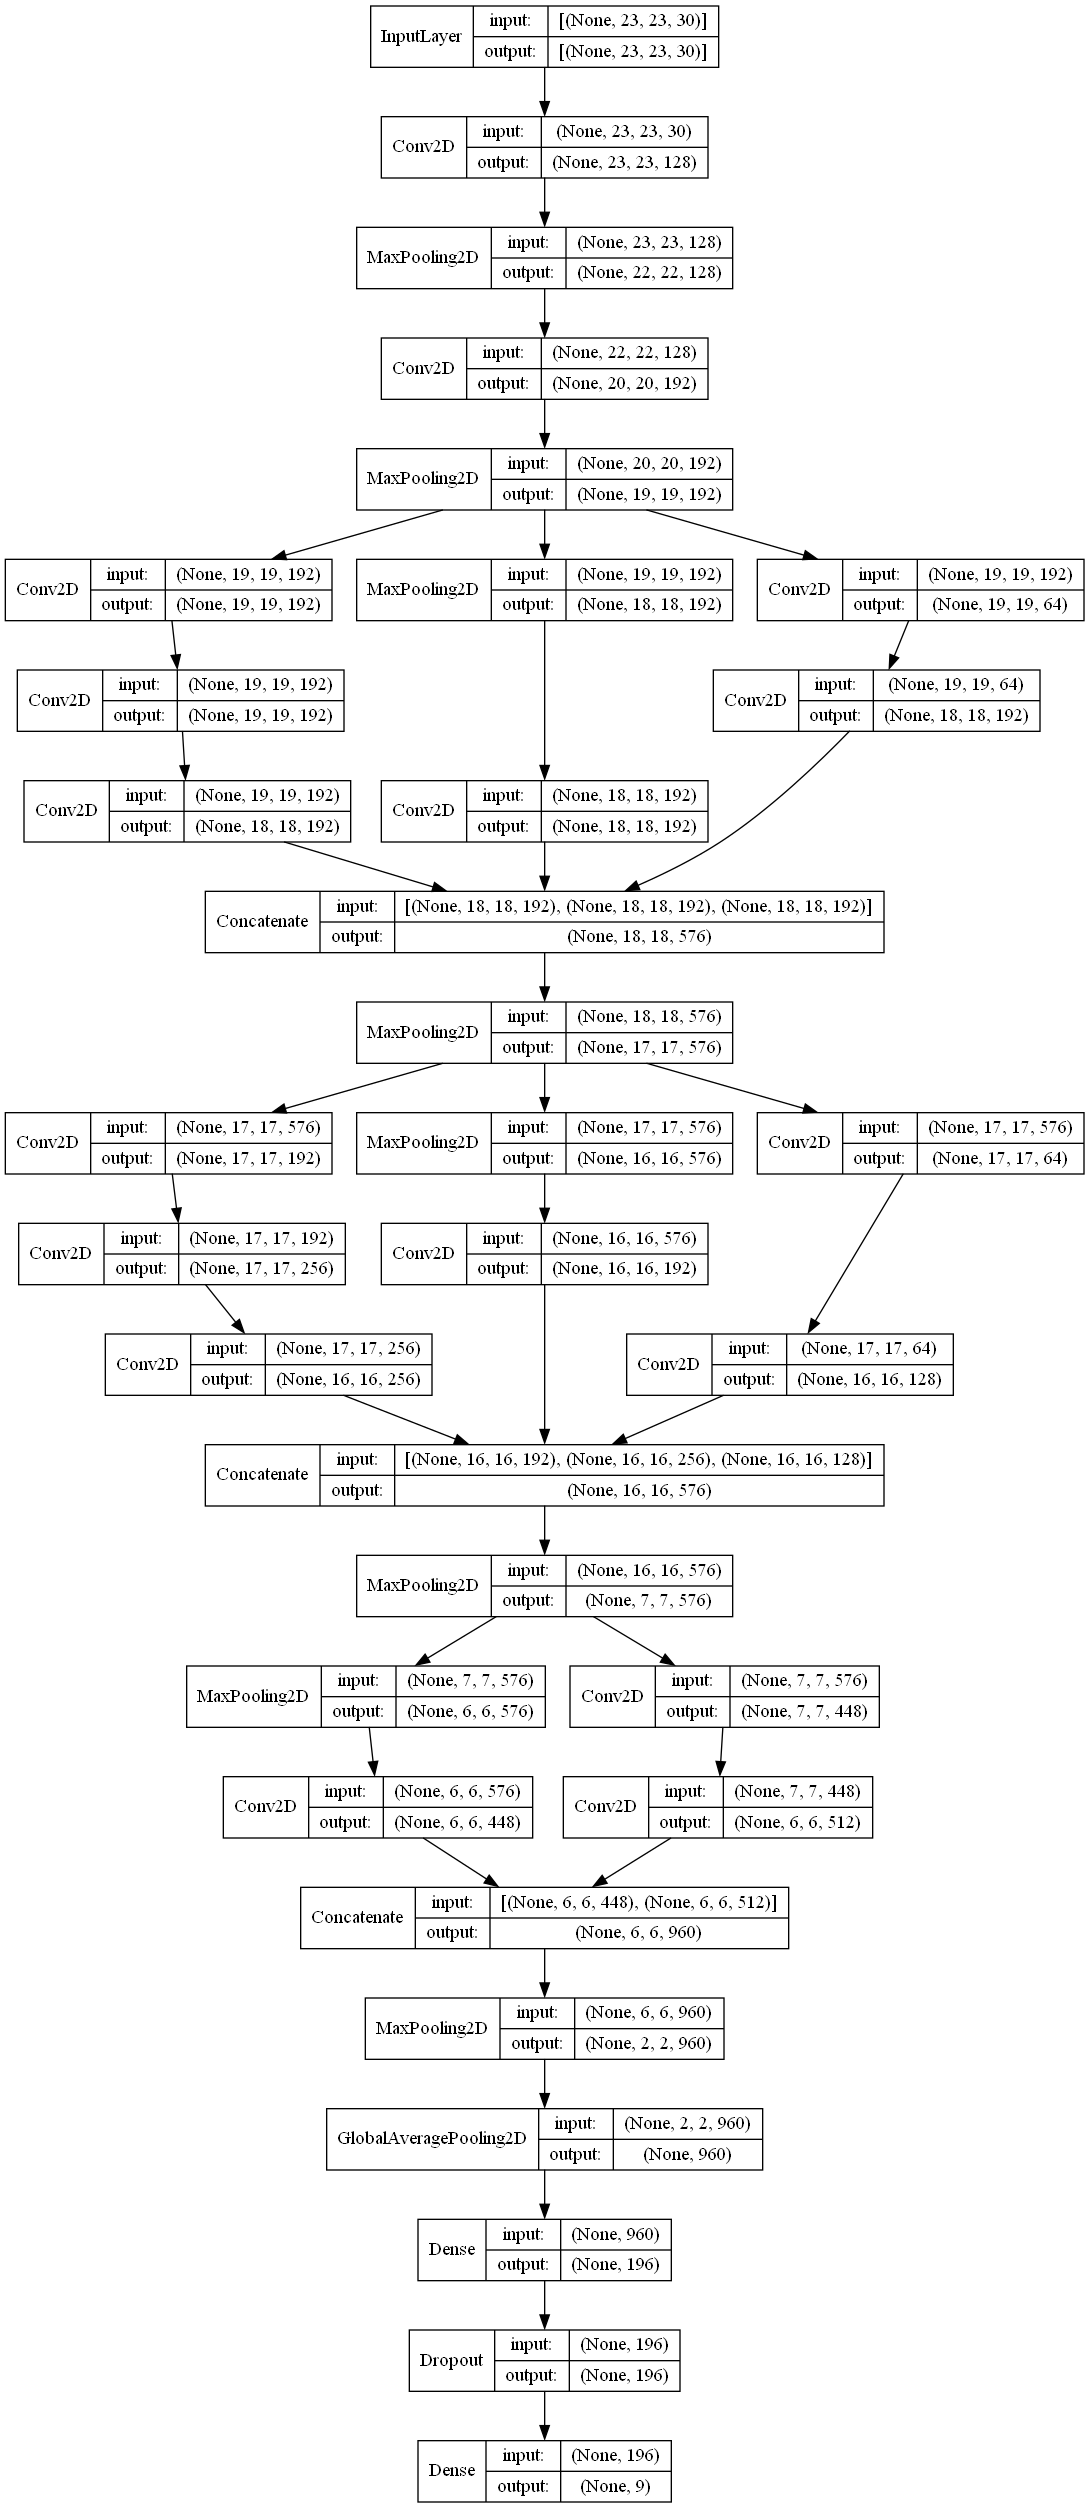
\includegraphics[width=\linewidth]{figs/vineyard_classification/networks/lt_cnn_23x22_64.png}
	\caption{CNN architecture proposed by Liu et al. \cite{liu_plant_2022} as implemented in this study to establish a comparison. }
	\label{fig:lt_cnn}
\end{figure}

\begin{figure}[bp]
    \centering
    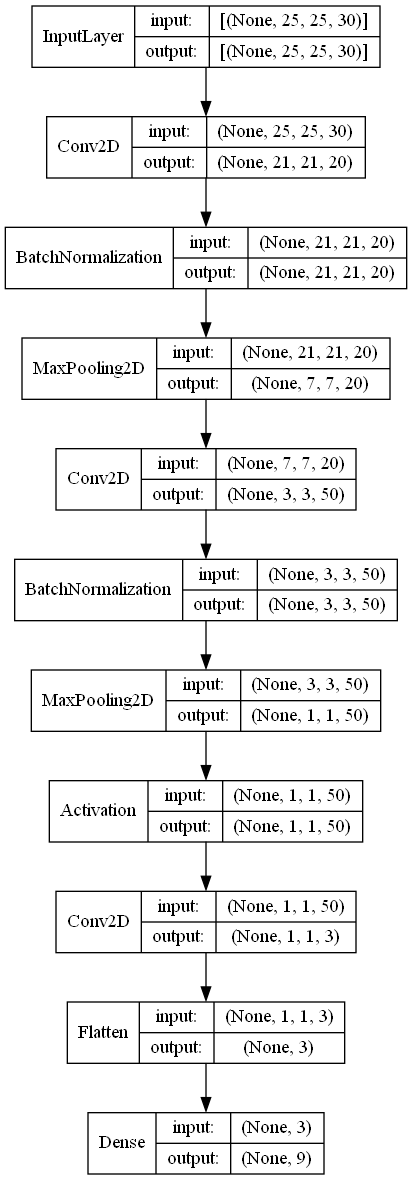
\includegraphics[width=\linewidth]{figs/vineyard_classification/networks/nezami_25x24_20.png}
	\caption{CNN architecture proposed by Nezami et al. \cite{nezami_tree_2020} as implemented in this study to establish a comparison. }
	\label{fig:nezami_cnn}
\end{figure}

\begin{figure*}[ht]
    \centering
    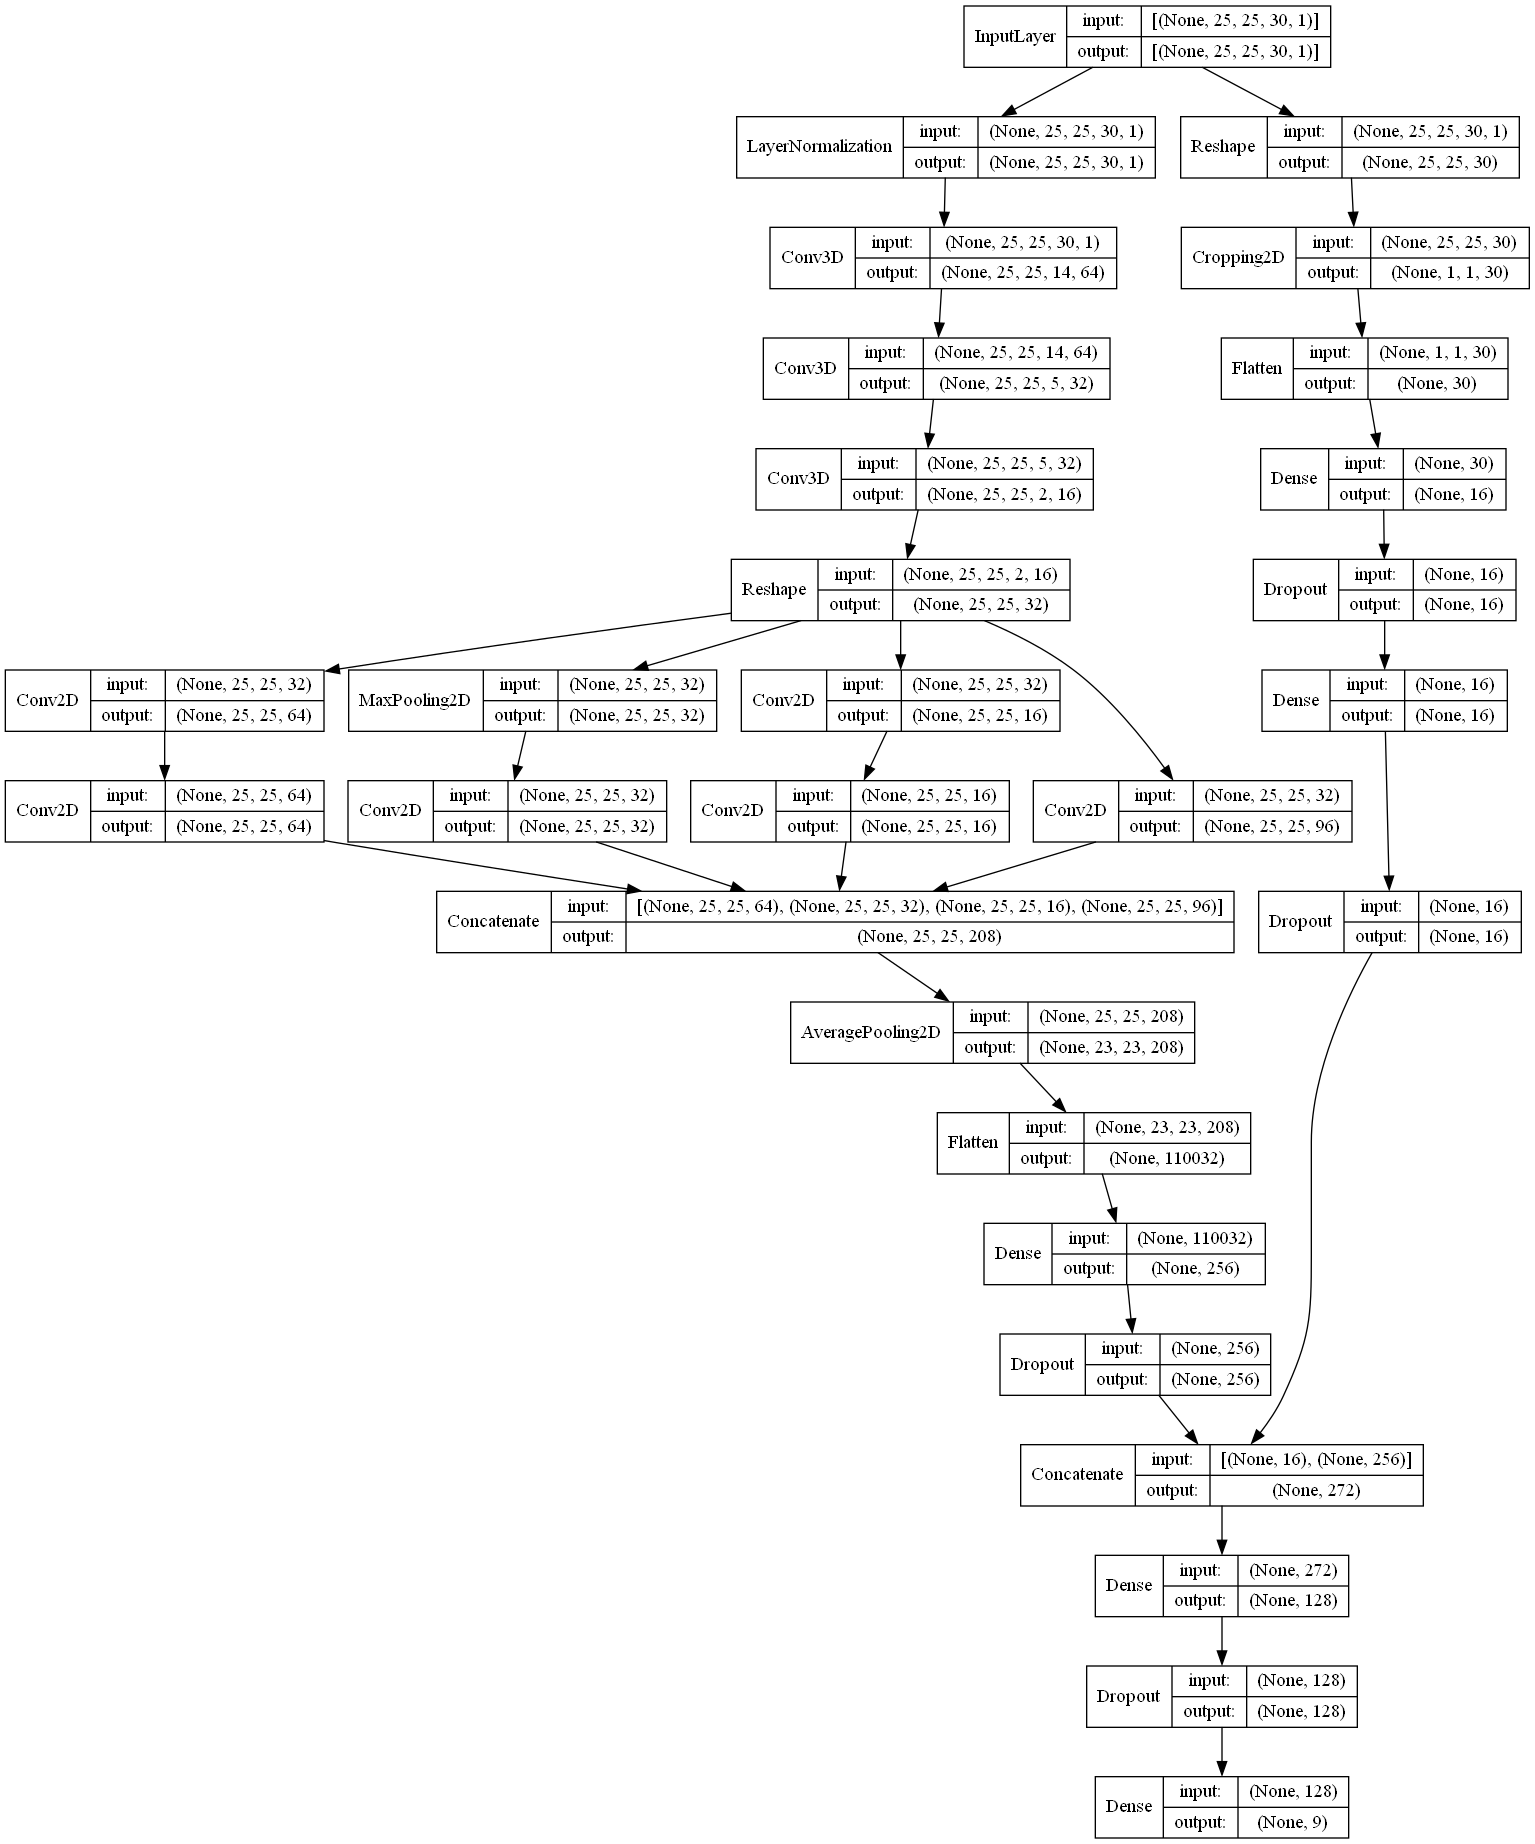
\includegraphics[width=\linewidth]{figs/vineyard_classification/networks/jigsaw_hsi_25x24_0.png}
	\caption{CNN architecture proposed by Moraga and Duzgun \cite{moraga_jigsawhsi_2022} as implemented in this study to establish a comparison. }
	\label{fig:jigsaw_cnn}
\end{figure*}

\begin{figure*}[ht]
    \centering
    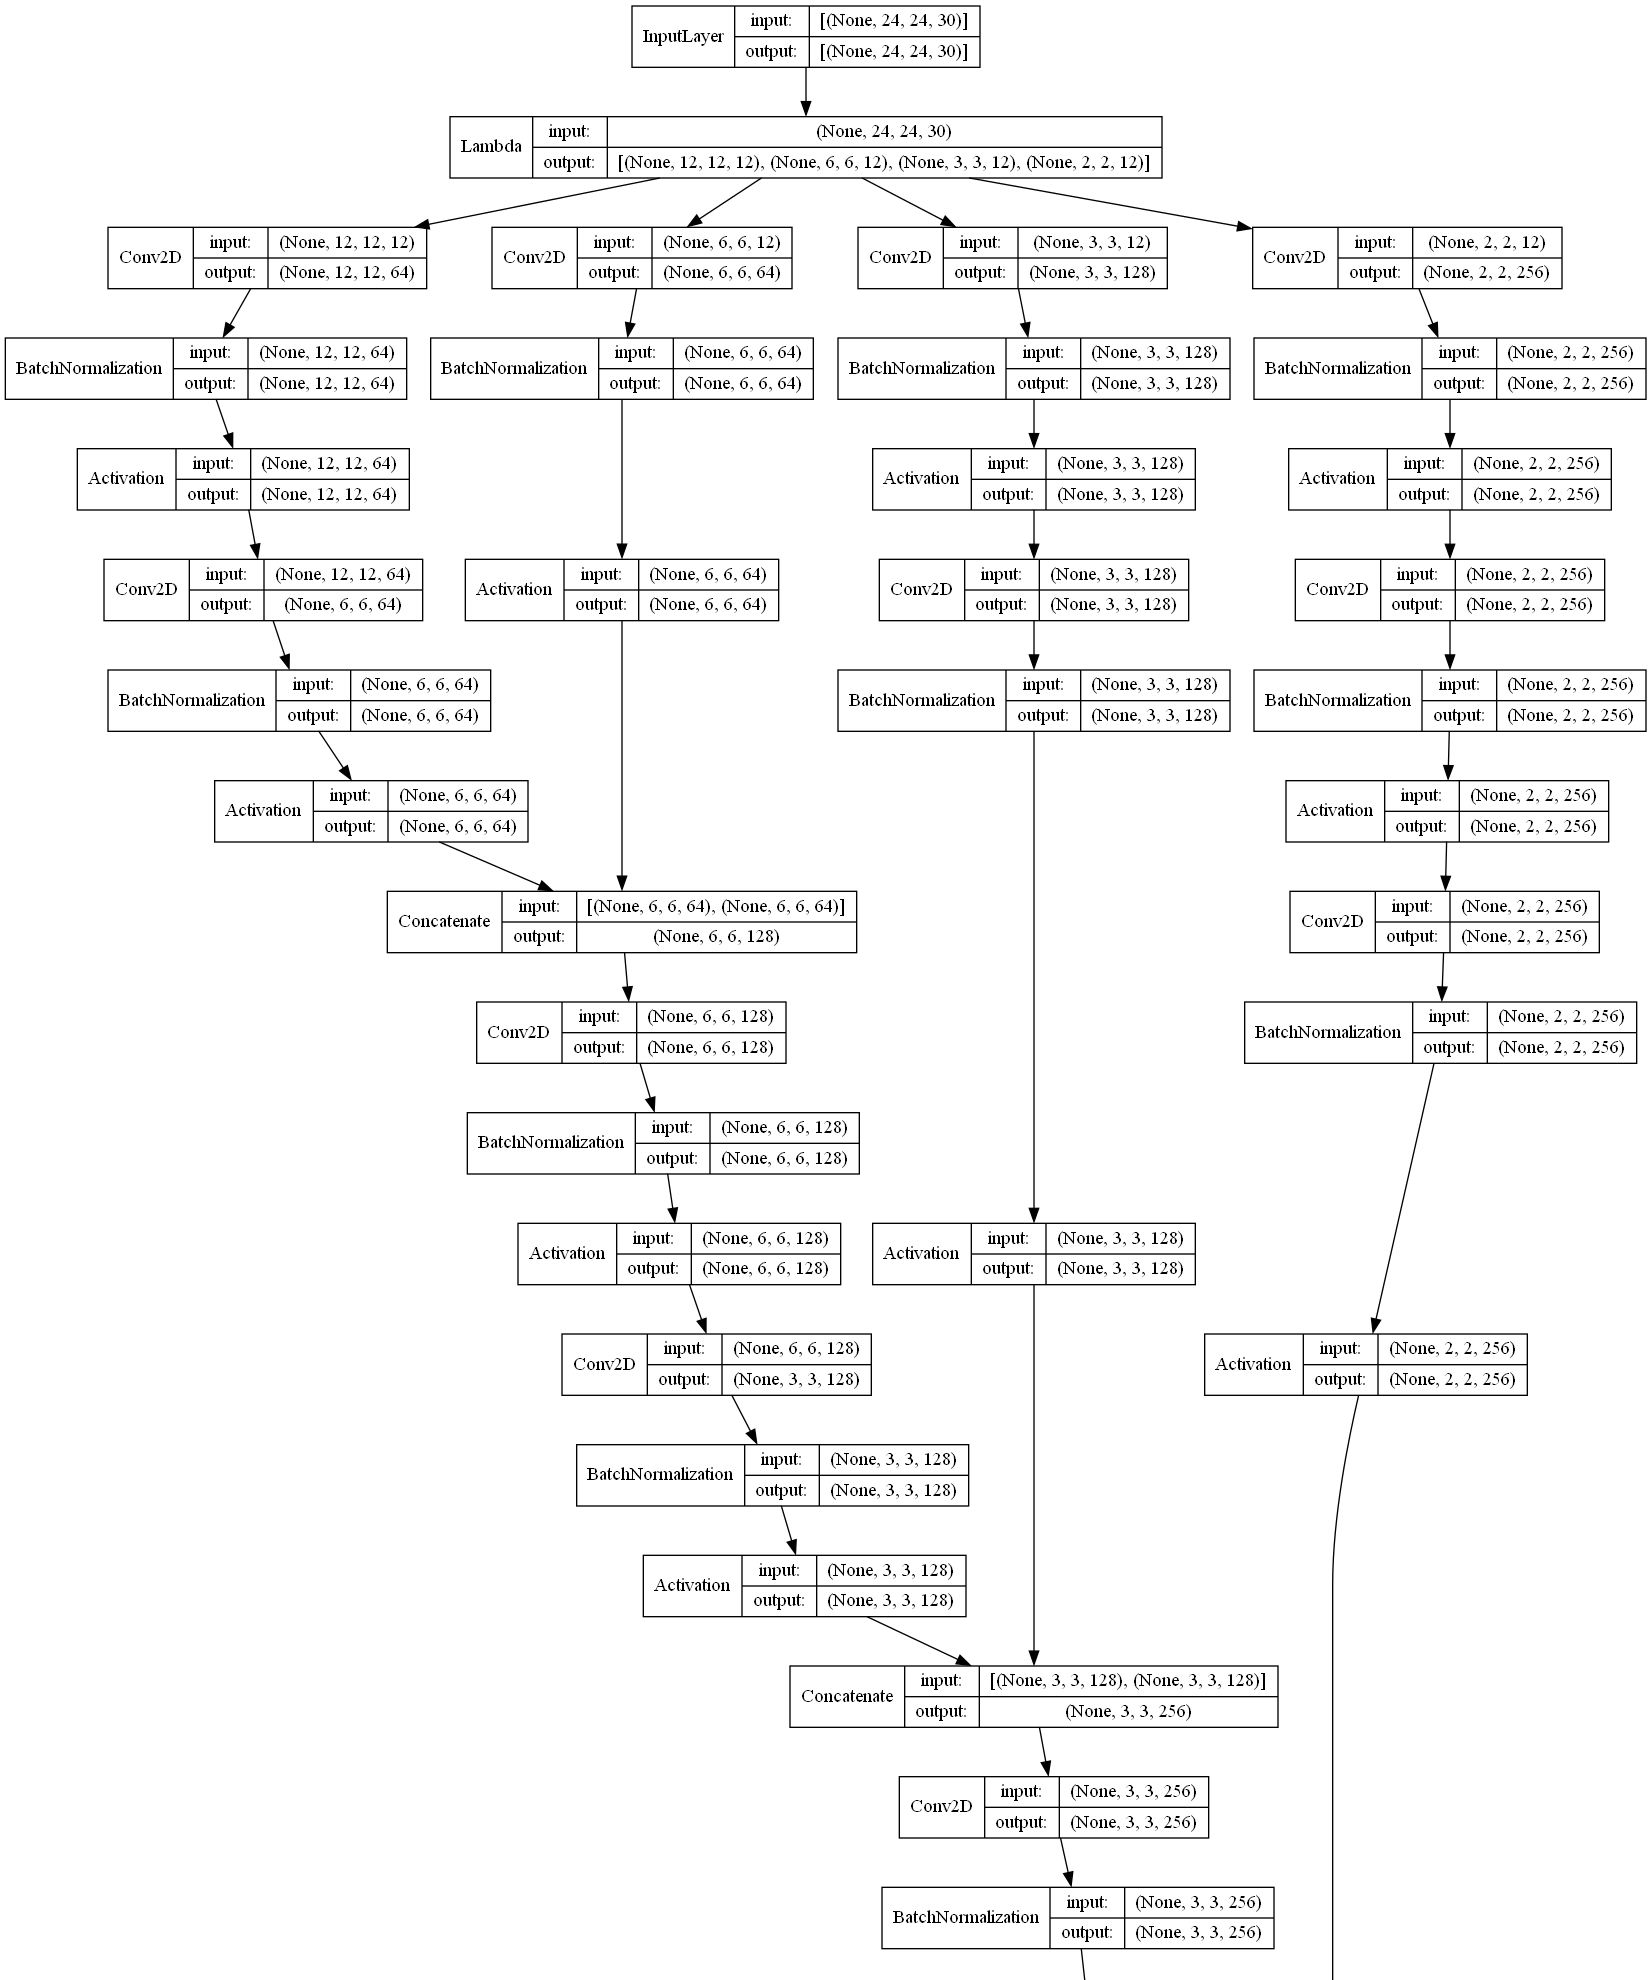
\includegraphics[width=\linewidth]{figs/vineyard_classification/networks/spectral_net_24x23_64_01.png}
	\caption{CNN architecture proposed by Chakraborty and Trehan \cite{chakraborty_spectralnet_2021} as implemented in this study to establish a comparison. }
	\label{fig:spectralnet_cnn}
\end{figure*}

\begin{figure*}[ht]
    \ContinuedFloat
    \centering
    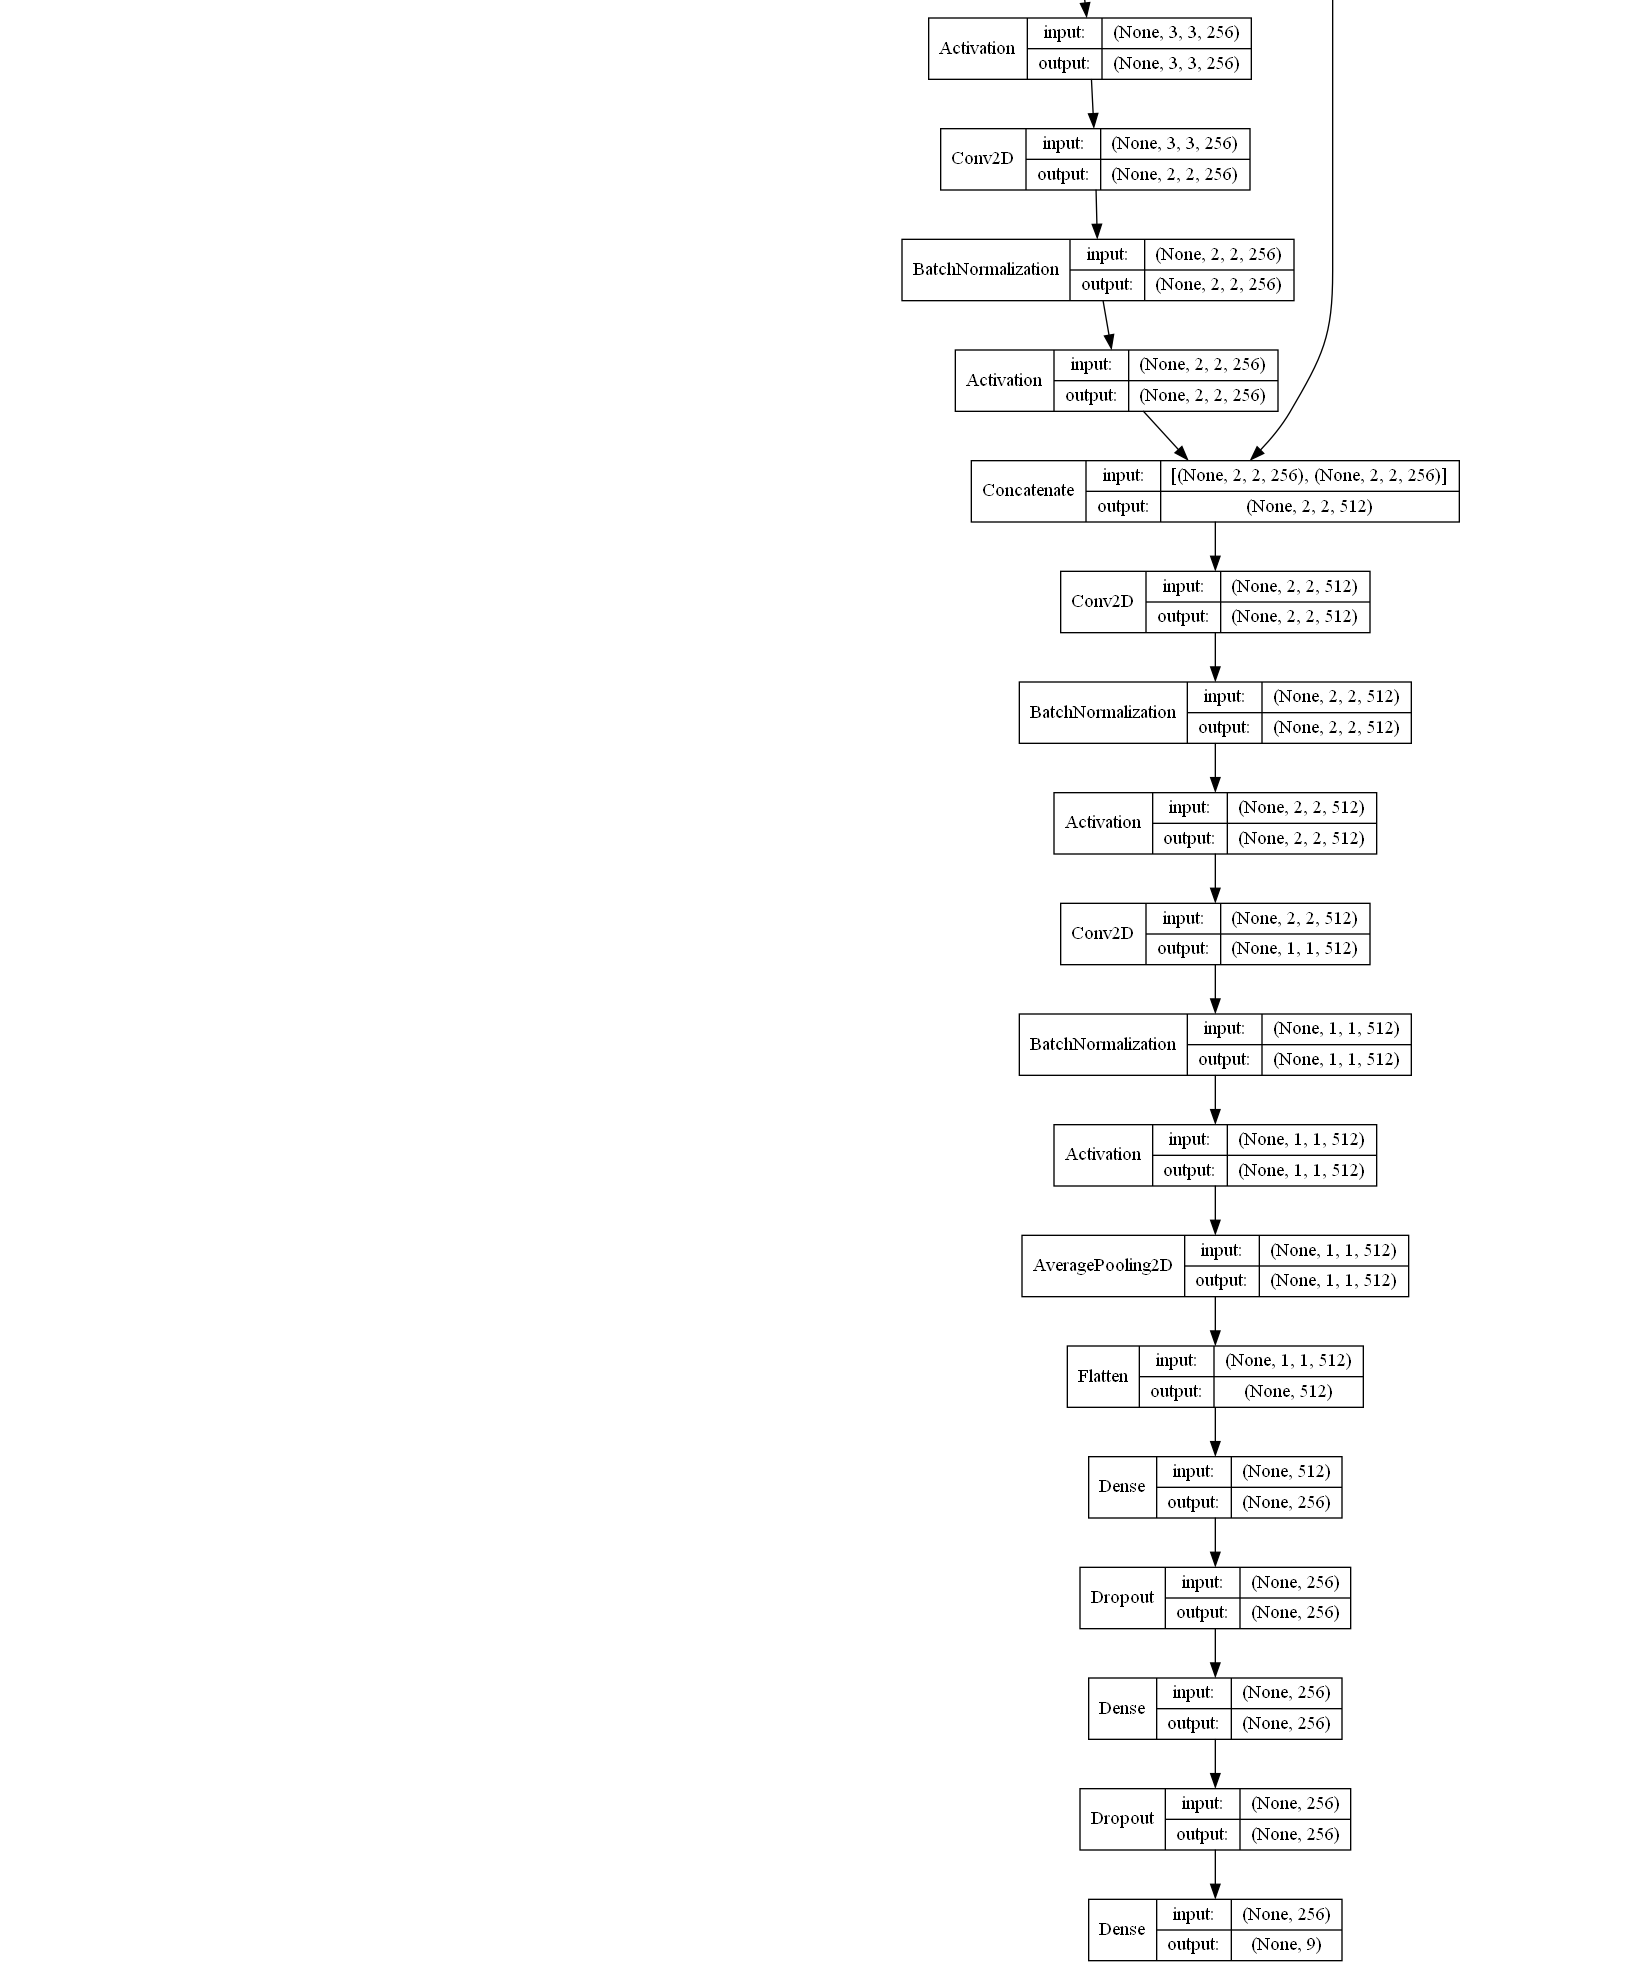
\includegraphics[width=\linewidth]{figs/vineyard_classification/networks/spectral_net_24x23_64_02.png}
	\caption{Continuation of Figure \ref{fig:spectralnet_cnn}. }
	\label{fig:spectralnet_cnn_continuation}
\end{figure*}

\begin{figure}[bp]
    \centering
    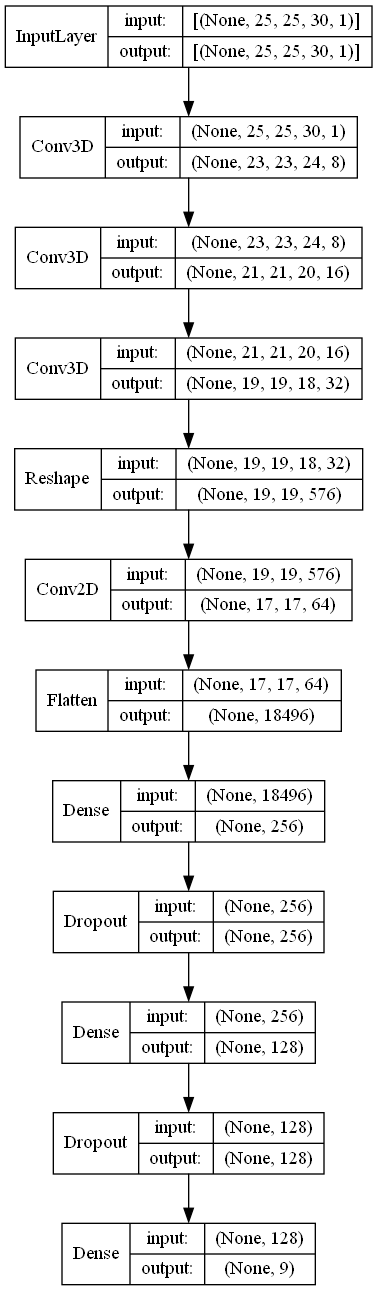
\includegraphics[width=\linewidth]{figs/vineyard_classification/networks/hybrid_sn_25x24_8.png}
	\caption{CNN architecture proposed by Roy et al. \cite{roy_hybridsn_2020} as implemented in this study to establish a comparison. }
	\label{fig:hybridsn_cnn}
\end{figure}